%% This is file `elsarticle-template-2-harv.tex',
%%
%% Copyright 2009 Elsevier Ltd
%%
%% This file is part of the 'Elsarticle Bundle'.
%% ---------------------------------------------
%%
%% It may be distributed under the conditions of the LaTeX Project Public
%% License, either version 1.2 of this license or (at your option) any
%% later version.  The latest version of this license is in
%%    http://www.latex-project.org/lppl.txt
%% and version 1.2 or later is part of all distributions of LaTeX
%% version 1999/12/01 or later.
%%
%% The list of all files belonging to the 'Elsarticle Bundle' is
%% given in the file `manifest.txt'.
%%
%% Template article for Elsevier's document class `elsarticle'
%% with harvard style bibliographic references
%%
%% $Id: elsarticle-template-2-harv.tex 155 2009-10-08 05:35:05Z rishi $
%% $URL: http://lenova.river-valley.com/svn/elsbst/trunk/elsarticle-template-2-harv.tex $
%%
%\documentclass[preprint,authoryear,12pt]{elsarticle}

%% Use the option review to obtain double line spacing
%% CHANGE FOR REVIEW!!
%\documentclass[authoryear,preprint,review,12pt]{elsarticle}

%% Use the options 1p,twocolumn; 3p; 3p,twocolumn; 5p; or 5p,twocolumn
%% for a journal layout:
\documentclass[final,authoryear,1p,times]{elsarticle}
%% \documentclass[final,authoryear,1p,times,twocolumn]{elsarticle}
%% \documentclass[final,authoryear,3p,times]{elsarticle}
%% \documentclass[final,authoryear,3p,times,twocolumn]{elsarticle}
%% \documentclass[final,authoryear,5p,times]{elsarticle}
%% \documentclass[final,authoryear,5p,times,twocolumn]{elsarticle}

%% if you use PostScript figures in your article
%% use the graphics package for simple commands
%% \usepackage{graphics}
%% or use the graphicx package for more complicated commands
 \usepackage{graphicx}
%% or use the epsfig package if you prefer to use the old commands
%% \usepackage{epsfig}

%% The amssymb package provides various useful mathematical symbols
\usepackage{amssymb}
%% The amsthm package provides extended theorem environments
%\usepackage{amsthm}

%% The lineno packages adds line numbers. Start line numbering with
%% , end it with \end{linenumbers}. Or switch it on
%% for the whole article with \linenumbers after \end{frontmatter}.
%\usepackage{lineno}


% NOTE: packages added for this paper
\usepackage{color}
\usepackage{latexsym}
\usepackage{mathtools}
\usepackage{amsmath}
\usepackage{amsthm}
\usepackage{listings}
\usepackage{longtable}
\usepackage{hyperref}
\usepackage{tabularx}
\usepackage{array}
%\usepackage[utf8]{inputenc} 
\usepackage{verbatim}

\renewcommand{\arraystretch}{1}
\pagestyle{plain}

\newtheorem{Axiom}{Axiom}
\newtheorem{definition}{Definition}
\newtheorem{theorem}{Theorem}
%\newtheorem{Definition Schema}[definition]{Definition Schema}

\definecolor{darkyellow}{RGB}{238,183,23}
\newcommand{\reminder}{\colorbox{darkyellow}}
\lstset{aboveskip=0.4cm, belowskip=0.4cm, belowcaptionskip=0.3cm, firstnumber=last, language=R, showspaces=false,showstringspaces=false,breaklines=true}
\hypersetup{%
    colorlinks=true, linktocpage=true, pdfstartpage=3, pdfstartview=FitV,%
    breaklinks=true, pdfpagemode=UseNone, pageanchor=true, pdfpagemode=UseOutlines,%
    plainpages=false, bookmarksnumbered, bookmarksopen=true, bookmarksopenlevel=1,%
    hypertexnames=true, urlcolor=blue, linkcolor=blue, citecolor=blue}

\renewcommand\arraystretch{1.0}


%% natbib.sty is loaded by default. However, natbib options can be
%% provided with \biboptions{...} command. Following options are
%% valid:

%%   round  -  round parentheses are used (default)
%%   square -  square brackets are used   [option]
%%   curly  -  curly braces are used      {option}
%%   angle  -  angle brackets are used    <option>
%%   semicolon  -  multiple citations separated by semi-colon (default)
%%   colon  - same as semicolon, an earlier confusion
%%   comma  -  separated by comma
%%   authoryear - selects author-year citations (default)
%%   numbers-  selects numerical citations
%%   super  -  numerical citations as superscripts
%%   sort   -  sorts multiple citations according to order in ref. list
%%   sort&compress   -  like sort, but also compresses numerical citations
%%   compress - compresses without sorting
%%   longnamesfirst  -  makes first citation full author list
%%
%% \biboptions{longnamesfirst,comma}

% \biboptions{}

\journal{Environmental Modelling \& Software}

\begin{document}

\begin{frontmatter}

%% Title, authors and addresses


\title{Meaningful Spatial Prediction and Aggregation}


\address[ifgi]{Institute for Geoinformatics, University of Muenster, Heisenbergstr. 2, 48149 Muenster, Germany}
\address[52n]{52° North Initiative for Geospatial Open Source Software GmbH, Martin-Luther-King-Weg 24, 48151 Muenster, Germany}

\author[ifgi]{Christoph Stasch\corref{cor1}}
\ead{staschc@uni-muenster.de}
\author[ifgi]{Simon Scheider}
\ead{s\_sche30@uni-muenster.de}
\author[ifgi,52n]{Edzer Pebesma}
\ead{e.pebesma@uni-muenster.de}
\ead{pebesma@52north.org}
\author[ifgi]{Werner Kuhn}
\ead{kuhn@uni-muenster.de}

\cortext[cor1]{Corresponding author. Current affiliation: Institute for Geoinformatics, University of Muenster, Weseler Strasse 253, 48151 Muenster, Germany. Tel.: +49 251 8331965. Fax.: +49 251 8339763}

\begin{abstract}
The appropriateness of spatial prediction methods such as Kriging, or aggregation methods such as summing observation values over an area, is currently judged by domain experts using their knowledge and expertise. In order to provide support from information systems for automatically discouraging or proposing prediction or aggregation methods for a dataset, expert knowledge needs to be formalized. This involves, in particular, knowledge about phenomena represented by data and models, as well as about underlying procedures. In this paper, we introduce a novel notion of \textit{meaningfulness} of prediction and aggregation. To this end, we present a formal theory about spatio-temporal variable types, observation procedures, as well as interpolation and aggregation procedures relevant in Spatial Statistics. Meaningfulness is defined as correspondence between functions and data sets, the former representing \textit{data generation procedures} such as observation and prediction. Comparison is based on \textit{semantic reference systems}, which are types of potential outputs of a procedure. The theory is implemented in higher-order logic (HOL), and theorems about meaningfulness are proved in the semi-automated prover Isabelle. The type system of our theory is available as an Ontology Web Language (OWL) pattern for use in the Semantic Web. In addition, we show how to implement a data-model recommender system in the statistics tool environment R. We consider our theory groundwork to automate semantic interoperability of data and models. 
\end{abstract}

\begin{keyword}
Meaningfulness \sep Knowledge-based Environmental Modelling \sep Spatial Statistics \sep Spatial Prediction \sep Spatiotemporal Aggregation
\end{keyword}

\end{frontmatter}

%\linenumbers

%% main text

\section{Introduction} \label{intro}

%added in revision
Summing temperature measurements or interpolating point source emissions is not meaningful. This paper formalises meaningfulness of applying prediction and aggregation procedures to data. With ever increasing data volumes \citep{Bell2009} of diverse origin and nature \citep{Parsons2011}, we observe an increase in importance of {\em information semantics} to the application of spatial statistics and environmental modelling \citep{Villa2009}. Although we do have access to more and more data, the distance between those who collect the data and those who analyze it has become larger. Also, in interdisciplinary settings, data from heterogeneous sources are combined by researchers without specific domain knowledge, increasing the risk of {\em inappropriate analysis} \citep{Pebesma2011}. Making sense of these large data volumes exceeds the limits and competence of a particular group of scientists \citep{Weinberger011}, and thus there is a need for \textit{semantic metadata} that can bridge the gap of knowledge which exists between groups \citep{Gray.2005}. 

NASA has recently argued that model reuse and \textit{data-model interoperability} has a significant added value, as about \textit{60\% }of the time of NASA scientists is spent on making data and models compatible \citep{NASA.2011}. In order to achieve integrated environmental modeling, standards that allow to describe and publish data and models in an automated fashion need to be developed \citep{Laniak2013}. When integrating environmental models, it is crucial to avoid ``constructs that are perfectly valid as software, but ugly or even useless as models''. \citep[p.149]{Voinov2013}. 

Observations form the basis of empirical and physical sciences. They provide samples for a process of interest, enabling us to infer knowledge about this process and to evaluate assumptions and hypotheses. In order to infer knowledge or test hypotheses about a process, \textit{statistical models and procedures} can be applied to observations. The syntactical integration of observations in statistical modeling frameworks is not an issue \citep{R}. However, the semantic integration of observations in such systems still forms a major challenge \citep{Sheth2008}, since not all syntactically possible applications are meaningful. Although there are already ontologies for describing observable properties and sensing devices such as the NASA SWEET ontologies\footnote{The SWEET ontologies are accesible at \url{http://sweet.jpl.nasa.gov/ontology/}.} or the W3C SSN ontology \citep{Compton2012}, a formalization of analysis procedures is missing. In this paper, we address the challenge of meaningful interpolation of a set of environmental observations and of meaningful aggregation in space and time. While there are sophisticated methods for interpolation and aggregation, such as Kriging \citep{Journel1978}, determining \textit{which} method is appropriate for \textit{which} kind of data in an automated fashion is an open research question. 

\begin{figure}[ht]
	\centering
		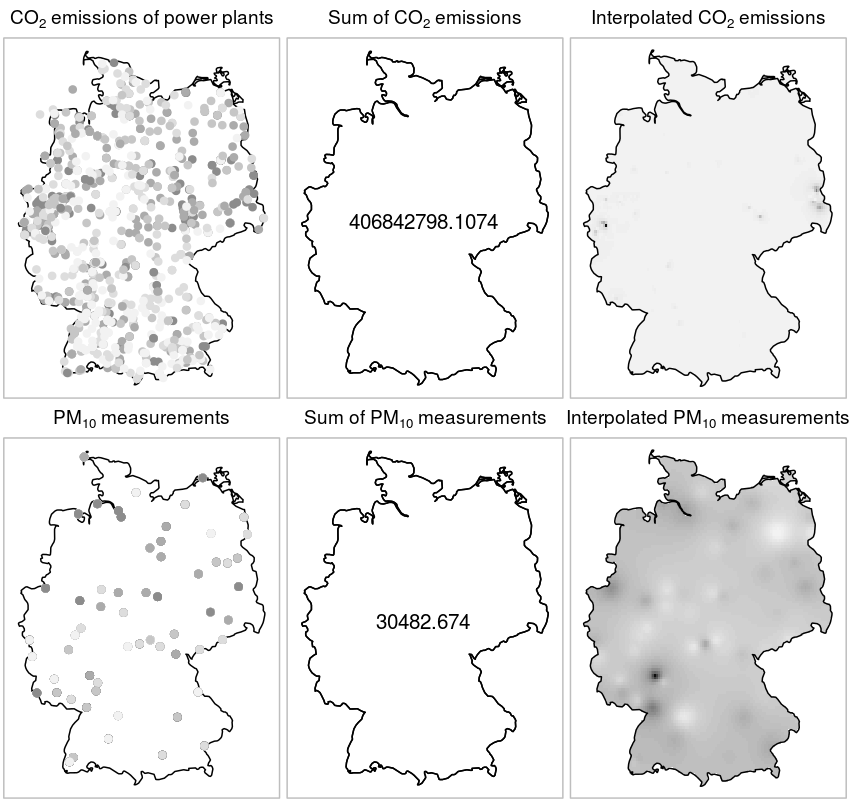
\includegraphics[width=12cm]{intro.png}
	\caption{Example datasets containing total $CO_2$ emissions of power plants in 2007 (upper left) and $PM_{10}$ measurements at 7th June 2005 (lower left). Both datasets consists of records of scalar values indexed by coordinates in space and can be easily spatially interpolated. However, the interpolated $CO_{2}$ emissions (upper right) can hardly be interpreted at locations where no power plants are located.}
	\label{fig:intro}
\end{figure} 

To illustrate the problem, consider two real datasets from the atmospheric domain shown in Figure \ref{fig:intro}: (i) total emissions of ${\it CO_2}$ for the year 2007 from power plants in Germany\footnote{The data is accessible for free at \url{http://www.carma.org}.} and (ii) daily mean concentrations of fine dust (${\it PM_{10}}$) measured at air quality stations in Germany\footnote{The data is available at \url{http://www.eea.europa.eu/themes/air/airbase}.}. Both datasets have an indistinguishable data structure: records of scalar values indexed by points in space and time. Hence, the datasets are often treated as the same in spatial analysis. However, though both datasets can be easily interpolated spatially (right column of Figure \ref{fig:intro}), interpolation of points is only \textit{meaningful} for ${\it PM_{10}}$ concentration and not for total emissions of ${\it CO_2}$ from power plants. Users unaware of the data semantics may apply inappropriate procedures because they do not distinguish between datasets with equivalent structure representing incommensurable phenomena. 
A comparable problem concerns the application of \textit{statistical measures} in spatio-temporal aggregation, such as summing up observation values within spatial regions. Computing the sum of the total ${\it CO_2}$ emissions of power plants over Germany may be meaningful, while the sum of ${\it PM_{10}}$ concentrations over an area may not. 

Though basic prediction and aggregation functionality for spatial data is often available in Geographical Information System (GIS) or statistical software in an adhoc fashion, the choice of a particular method is usually up to the user and its appropriateness is not checked by the system. Furthermore, while measurements scales \citep{Stevens1946,Suppes1967,Chrisman1995} are well established, in many cases, allowable operations are unknown for a dataset. It is, e.g., not meaningful to compute the mean value of a numerical ordinal variable, although it is possible from a computational viewpoint. 

We argue that the problem of meaningful prediction and aggregation requires knowledge about the \textit{meaning of data}, i.e., \textit{semantic knowledge}, in machine readable form to help users determine which prediction or aggregation method can be applied to which dataset. In this paper, we suggest a way how the notion of meaningulness can be operationalized:
\begin{enumerate}
\item Formal specifications make some of the knowledge underlying meaningful statistics more explicit and readable for machines.
\item In a rough approximation, a statistical prediction or aggregation method can be said to be meaningfully applicable to a data set, if it is \textit{semantically interpretable} in the observation context of the data. This context can be captured, to a significant degree, by \textit{(semantic) reference systems} \citep{Kuhn2003}.
\item On this basis, the well-known conceptual distinction between \textit{(marked) point pattern}, \textit{geostatistical variables} and \textit{lattice data} \citep{Illian2008,Burrough1998,Cressie2011}, can be made formally explicit.
	\item Meaningfulness of prediction can then be checked by testing whether \textit{prediction functions} underlying statistical models \textit{formally correspond} to \textit{observation functions} underlying data, where both are typed by semantic reference systems.
	\item Meaningfulness of summation can be checked by testing whether regions over which the data is aggregated formally correspond to the \textit{observed window} of the data to be aggregated.	
	\item This shows a way to design a recommender tool in Spatial Statistics\footnote{In this paper, we follow the distinction introduced by \citep{Cressie2011}, where statistics refers to summaries\\ of data and Statistics to the Statistical Science. The same is applied to Spatial Statistics and Geostatistics.}, in which data and variables can be linked to interpolation and aggregation methods. 
\end{enumerate}

The contribution of this paper is a formalisation of meaningfulness of spatial prediction and aggregation with respect to datasets. Out of scope are the semantic description of observable properties, of statistical models, and of application problems. We make the case for our notion of meaningfulness based on the two scenarios from the atmospheric domain introduced above (air quality and $CO_2$ emissions). We test our theory and prove meaningfulness in Isabelle/HOL, a higher-order theorem prover. A preliminary Web Ontology Language (OWL) pattern, which can be used by statistical applications on the Web, and a prototypical implementation in R illustrate some of its potential.

The remainder of this paper is structured as follows. The next section
introduces the background of our work including overviews on Spatial Statistics, on spatio-temporal aggregation, on meaningfulness in measurement theory, and on semantic reference systems. Afterwards our functional approach to formalize spatial statistical knowledge is described in detail. Then, a description of a prototypical implementation, an R package that extends the package sp, is introduced. Finally, after discussion of our approach, conclusions and directions for future research are presented. 

\section{Background} \label{background}

This section provides background and a preliminary discussion of the problem of meaningfulness. First, basic variable types are introduced which are relevant for meaningful Spatial Statistics. Then, we describe our notion of spatio-temporal aggregation. Afterwards, we discuss the definition of meaningfulness in measurement theory. Finally, semantic reference systems for space, time, as well as for thematic domains are described, and it is argued why they are useful for making the necessary distinctions. 

\subsection{Spatial Statistics}
\label{spatStat}

Spatial Statistics \citep{ripley81,cressie93,Cressie2011} is a branch of Statistics that deals with spatial and spatio-temporal processes. Although all observations are taken under circumstances that can be characterized by a location and time, in many cases location and time do play a minor role, for instance where controlled experiments in lab conditions eliminate the role of space and time. In case of medical experiments, the subject's identity and age may form the major reference. However, when observations are taken outside a lab, non-controllable factors typically cause them to be correlated in space and/or over time. Spatial Statistical models address such correlations, allow inferences, and are used for the prediction of phenomena in space and time.

For spatio-temporal processes, \citet{Cressie2011} use the following notation: 
\begin{equation}
Z(s), \ s \in W, \ W \subset \mathbb{R}^d 
\label{eq:st}
\end{equation}
with $Z(s)$ an observed or unobserved value at $s$, the combination of spatial location and time; $W$ the spatial and temporal domain or window over which $Z$ is defined; and $d$ the dimensionality of space-time (e.g. three in case of two-dimensional space plus time). The location $s$, the spatial and/or temporal \textit{support}, is a region in a spatial and/or temporal reference system and may be represented as a point.

Two basic forms can be distinguished. First, $Z$ is defined for every possible value of $s$ (hence Z is total). In Geostatistics, one assumes that s is a continuous index. In this case, $Z(s)$ is a {\em geostatistical} variable, and the challenge often lies in predicting values $Z$ for unobserved locations $s_0$, based on a limited set of $n$ observations $Z(s_1),...,Z(s_n)$. 

The second form is that of {\em point pattern} variables \citep{Illian2008}, where not for every point $s_i$ Z is defined (hence Z is partial).  A pure point pattern consists {\em only} of those locations. {\em Marked point patterns} include the Z values (the marks).  Typical questions in point pattern modelling are whether point density variations can be considered random, whether points interact (e.g., attract or repulse), and how point density, interactions, or marks depend on known covariates. For analyzing point pattern data, it is important to know the observation window $W$ \citep{Baddeley2005}, as the latter allows discriminating between where we know there are no points from where nothing is known.

If values are considered results of a random process, the values cannot be chosen arbitrarly and we call that variable a \textit{random variable}. In contrast, we call a variable a \textit{fixed variable}, if the values can be fixed, i.e. the values can be selected arbitrarly. Point pattern analysis consider $s=s_1,...,s_n$ as a {\em random set}, meaning that locations are random variables.  Given the locations, the marks of a marked point process $Z(s)$ are considered random variables. For geostatistical variables, only $Z$ is considered random, as observation and prediction locations $s$ can be chosen arbitrarily.

In the case of {\em Lattice data}, observed values reflect aggregations over a set of covering regions rather than (values for) points. The union of regions forms the area of study $W$.  The observed variable is usually modelled as a random field, the regions are not random.  Images are often considered as a special case of lattice data.  Typical problems are modelling spatial dependence, assessing whether spatial patterns might be completely random, and finding relations with covariates.

The challenge is to bring this knowledge into a semantically explicit, machine-readable form, which can be used for automated reasoning about meaningful application of methods to the various kinds of data.


\subsection{Spatio-temporal Aggregation}
\label{stagg}

Statistical measures are computed on aggregates of observations. \textit{Spatio-temporal aggregation} \citep{Jeong2004,VegaLopez2005,Stasch2012a} aggregates observations to some coarser spatial regions and/or temporal extents using some spatial or temporal grouping predicate, usually spatial or temporal regions. Then, an \textit{aggregation function} is applied to the observed values of each group in a spatial and/or temporal region. These regions are the supports of the aggregated values and indicate a \textit{change of support}. In this work, we focus on spatio-temporal aggregation processes where grouping predicates indicate selection of observations for point pattern or geostatistical variables within spatial and temporal regions and where aggregation functions are simple functions such as mean, sum or median.

A specific problem is using the sum as aggregation function. This problem is identified in the Online Analytical Processing (OLAP) and statistical database community as the summarizability problem \citep{Lenz1997,Mazon2009}, but has not yet been specifically investigated for the spatial domain. While in general, from the measurement theory viewpoint, the summation is meaningful as long as the measurement scale of the quality is interval or ratio scale, using the sum as an aggregation function is sometimes meaningful, but sometimes not. In this paper, we argue that observed values that are distributed in space can only be meaningfully summed, if we have complete knowledge about the extent over which values are summed. This may be the case for point patterns, but not for geostatistical data.

\subsection{Meaningfulness in Measurement Theory}
\label{measTheory}

As there are different notions of probability in statistical theory,  there are different approaches to meaningfulness in measurement theory that may lead to different statistical models and conclusions \citep{Hand1996}. In the representational approach, which is the most widely adopted, real world objects, their properties, and their relationships are modeled by empirical relational systems, and measurements are expressed as mappings from object properties to numbers in a numerical system \citep{Suppes1967}. 

Usually, empirical properties can be mapped to numerical systems in different ways, according to different measurement scales. For example, the length of an object can be expressed in meters or in inches. Transformations between such different numerical representations, which preserve the relationships of objects in the empirical system, are called \textit{permissible transformations}. Scale types of measurement are defined as classes of permissible transformations among numerical representations. In the length example, the length is of a ratio scale type since the permissible transformations are positive similarity transformations (multiplication with a scalar value).  

Stevens \citep{Stevens1946} introduced the notion of meaningfulness to Statistics. He defined four measurement scale types (nominal, ordinal, interval, ratio). Meaningful statistics are those that are invariant over permissible transformations of each scale type. As pointed out by many authors \citep{Chrisman1995,Suppes1967}, there are more practically relevant scale types than the ones defined by Stevens. For example, wind direction is usually provided on a cyclic scale (degrees from north axis). Furthermore, Adams \citep{Adams1966} emphasized that meaningfulness also depends on the context in which the statistics are used. 

We understand meaningful statistics and prediction in a more specific sense, which goes beyond the distinction of scale types and is rather located on the level of particular scales that allow to differentiate observed phenomena as well as underlying observation procedures. In our approach, statistical operations are meaningful with respect to data, if these operations are intepretable in the \textit{context in which the data was generated}. We use semantic reference systems to capture this pragmatic context.

\subsection{Semantic Reference Systems and Data Generation Procedures}
\label{semRefSystems}

According to \cite[p.35]{Berners-Lee2001},``The Semantic Web is not a separate Web but an extension of the current one, in which information is given well-defined meaning, better enabling computers and people to work in cooperation.'' Formalized knowledge, usually provided in the form of ontologies \citep{Gruber1993}, is used in the Semantic Web to support interoperability and to make documents discoverable, readable, and interpretable for machines. A common language for creating, exchanging, and publishing ontologies in the Web is the Web Ontology Language (OWL)\footnote{\url{http://www.w3.org/TR/owl2-overview/}}. The question now is which formal distinctions need to be captured in an ontology in order to formalize meaningfulness.  

Deciding about meaningfulness of data for certain prediction methods or descriptive statistics requires formal distinctions that safeguard the application or at least caution against an inappropriate choice. These distinctions need to go beyond well-understood mathematical abstractions of statistical theory to capture some of the \textit{meaning of the data} to which statistical models are to be applied. Regardless of whether the data is a product of prediction or observation, what makes it \textit{meaningful} to us is knowing how to \textit{interpret} it. This involves, essentially, knowing how to \textit{refer} to the phenomena underlying data in the context of its generation \citep{Scheider.2011c}. The latter competence is called \textit{reference} and involves knowledge about repeatable human and technical operations that allow to share phenomena, such as observation, abstraction and prediction procedures. Statistical inference and modelling critically depend on the observation and abstraction process itself, not only on the world that is being observed or on the cognitive and linguistic aspects of its representation. For example, a statistical model critically depends on the \textit{resolution} of the data sample, and this resolution is a consequence of certain observation and abstraction procedures \citep{Frank2009}. Therefore, we suggest to follow a \textit{pragmatic} approach to data semantics, requiring that the generation procedure needs to be somehow reflected in the semantic description of statistical data.

One approach to reference systems, in this pragmatic sense, are measurement scales. However, current ontologies about measurement scales, such as \citep{Rijgersberg2012}, are not sufficient for our purpose. The reason is that Statistics is not only (and only in limited cases) about measurable qualities. In particular, Spatial Statistics needs to refer to a wide range of other spatio-temporal phenomena, including discrete objects and events. Therefore a more general notion of a reference system is required. 

Semantic reference systems were first proposed by Kuhn \citep{Kuhn2003}. This concept generalizes spatial and temporal reference systems. Spatial reference systems are, for example, physically anchored mathematical ellipsoids that allow to unambiguously refer to locations on the earth surface. They are grounded in conventional standard directions and positions that geodesists can refer to. Semantic reference systems, as a generalization, are formal theories anchored in conventionally established observation procedures. They provide reference for arbitrary observable phenomena, also for phenomena described by complex geometries or attributes in a Geographic Information System (GIS). There are, e.g., reference systems for time in terms of calendars, for places in terms of postal addresses, as well as for other kinds of observable phenomena. For many spatio-temporal phenomena, such as geographic objects and events, reference systems can be constructed in a similar way, based on repeatable observation and abstraction procedures \citep{Scheider.2011c}. 

In this paper, we will just make use of the discriminative power of reference systems regarding domains of phenomena of interest, while the question of constructing and grounding them is not in focus. Therefore, we will presuppose that we have reference systems of an appropriate kind at our disposal, and we will preserve the term \textit{referent} to speak about an individualized phenomenon in the domain of a reference system. The meaning of the latter is conventionally established.

Since reference systems are formal theories grounded in repeatable procedures, their domain can be viewed as the structured set of all \textit{possible entities that can be the result of such a procedure}. For example, the set of all potentially observable colors makes a color space, or the set of all potentially observable locations makes a spatial reference domain. By a \textit{procedure}, we understand in this paper \textit{any conventionally shared instruction to generate %tuples of %
entities of a reference system}, in particular \textit{mathematical functions}. This is regardless of whether this instruction is explicit in the form of a computational rule, such as a prediction algorithm in geostatistics, or whether it is implicit in the form of human action schemes.

\section{A Formalization of Meaningful Prediction and Aggregation} 
\label{approach}

In this section, we introduce the formalism that enables to infer whether applications of prediction and aggregation procedures to datasets are meaningful, provided that their underlying observation procedures are known. First, an overview is given of the approach (section \ref{formOverview}), followed by an introduction to our formal notation (Section \ref{notationIsabelle}), and subsections for each core concept in our formalism (Sections \ref{refSystems}-\ref{aggregation}).

\subsection{Overview}
\label{formOverview}
The basic idea of our formalism is a formal distinction between \textit{representations of procedures as functions}, which capture knowledge about potential operations such as observing or predicting phenomena, and \textit{representations of data sets as predicates over function domains}, which denote limited (finite) results of applying such operations. This distinction allows us to compare data and procedures in terms of the underlying data generation capabilities. We explain this idea first in an informal way.
 
An observation procedure is an operational description how to observe a phenomenon. For example, the observation procedure for observing ${\it PM_{10}}$ involves localisation of the measurement device in space, time measurement by a clock, and the use of a ${\it PM_{10}}$ sensor, whose technical specification describes the measurement procedure in more detail. By executing this procedure, one takes unique measurements at arbitrary points in time and space. Therefore, we can specify the observation procedure by a continuous \textit{observation function}, a mapping from arbitrary locations and times to concentrations. Similarly to an observation procedure, a particular prediction procedure is specified by a \textit{prediction function} in our formalism. An example of a prediction procedure is the description of ordinary kriging in a statistical book \citep[p.145]{Cressie2011}, which can be specified as a function from continuous space and time to predicted values. Hence, our formalism consists of functional specifications, shown in yellow colour in Figure \ref{fig:overview}, which allow to distinguish the different types of Spatial Statistical variables: point pattern, marked point pattern, and geostatistical variables, in terms of different types of functions. 
 
The meaning of the functional domains and ranges, i.e., of the \textit{types of entities} being related by a function, is given in terms of reference systems shown as blue concept in Figure \ref{fig:overview}. More precisely, functions are mappings from certain reference domains to other ones, where the latter are specified as formal types. 

As an example, the function specifying ${\it PM_{10}}$ observations in Germany in the year 2008 is a mapping ${\it WGS84 \Rightarrow UTC2008 \Rightarrow PM_{10}}$ from the spatial reference domain given in the World Geodetic System 1984 (${\it WGS84}$), WGS84 coordinates in Germany, and the temporal reference domain ${\it UTC2008}$, the year 2008 in Universal Time Coordinated (UTC), to a sensor reference domain ${\it PM_{10}}$ defining concentration values in $\mu g/m^3$. Such an observation function is of a \textit{geostatistical type}, since it maps points in continuous space and time to quality values.

\begin{figure}[ht]
	\centering
		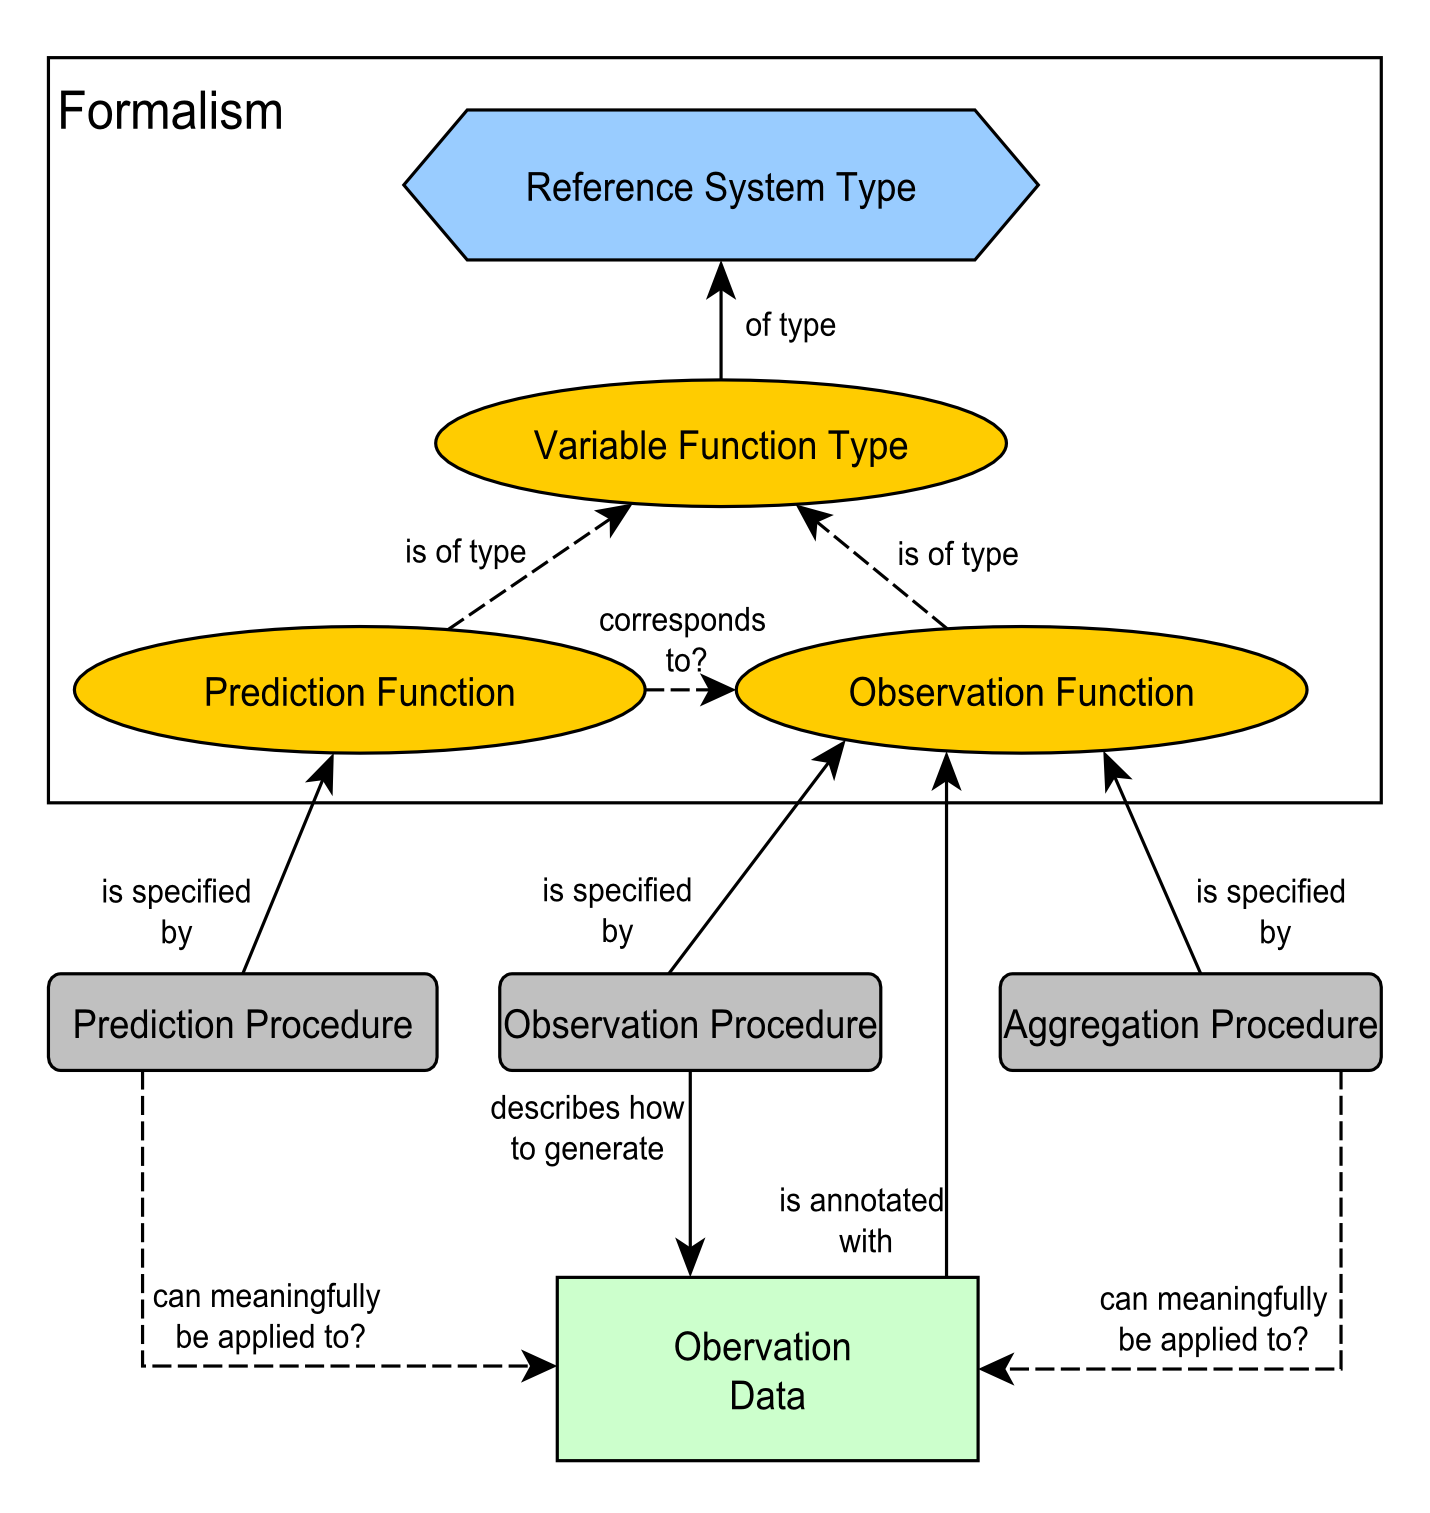
\includegraphics[scale=0.65]{overview.png}
	\caption{Overview on the approach of meaningful prediction and aggregation. Functional declarations are shown as yellow concepts, informal descriptions of prediction, observation and aggregation procedures as grey concepts, observation data as green concept and types as blue concepts. The arrows indicate explicit relations in our formalism. The bold lines represent correspondence checks for meaningfulness inside the formalism. The dotted arrows show implicit relations to concepts outside of our formalism.}
	\label{fig:overview}
\end{figure}

The observation procedure, which is specified as an observation function, stands for potential observations, whereas executing the procedure generates actual observations, i.e., \textit{data}. Since the procedure can be executed only finitely many times, data is always finite, in contrast to the corresponding observation function. However, annotating data with an observation function allows us to link it with the underlying observation procedure, and thus, to take possible observations into account when deciding about meaningfulness. More precisely, in order to check whether a prediction procedure can be meaningfully applied to a dataset, we propose to check whether the respective observation function corresponds in a certain sense to the prediction function which specifies the prediction procedure (compare Figure \ref{fig:overview}). 

How does this approach help us to distinguish the geostatistical from the point pattern scenario? Since the function formalism captures \textit{procedures} in the sense of \textit{potential} observations or predictions, it allows, for example, to capture the difference between continuously observable space and discretely observable objects, even though the actual datasets are discrete in both cases and, thus, may not be distinguishable. The difference between continuously observable space and discretely observable objects is, in essence, the difference between a geostatistical and a point pattern variable. Furthermore, a prediction function, which specifies \textit{what can be done} with a prediction procedure such as Kriging interpolation, can only be considered meaningful with respect to an observation dataset, if the underlying observation procedure supplies possible observations for each predictable case. For example, in the case of ${\it CO_{2}}$ emissions of power plants, a geostatistical interpolation generates values at locations where no power plants are located, and, hence, an interpolation of power plant emissions becomes meaningless.

In a similar way, the \textit{observed window}, which is the extent to which an observation dataset ``covers'' a spatio-temporal domain, can be used to determine whether an aggregation procedure can be meaningfully applied to a dataset or not. For example, since the observation of ${\it PM_{10}}$ cannot cover a continuous spatial aggregation region, such as the spatial region of Germany, by a discrete data sample, using the sum to aggregate this dataset is meaningless. However, summing up emissions from discrete power plants may be meaningful, provided that the observed window covers the whole region of Germany. Note that also in this case, the essential idea is that a specification of an observation procedure accounts for what can be observed in contrast to the limited sample of an actual dataset.

\subsection{Formal Notation and Semi-automated Test and Proof in Isabelle}
\label{notationIsabelle}

The formalism is written, implemented and tested in \textit{Isabelle/HOL}, a typed higher-order logic (HOL) which allows for reasoning over functions. Isabelle comes with a generic proof assistant which is available as jEdit plugin\footnote{\url{http://www.cl.cam.ac.uk/research/hvg/isabelle/}}, and which offers interactive syntax and type checking, as well as interactive proof support in natural deduction style. We adopted the notational style of Isabelle, since it follows ordinary conventions known from logic and mathematics books, and thus should be easily readable. Furthermore, we also tested and proved all our theorems with Isabelle\footnote{The Isabelle theory is available online at: \url{http://www.meaningfulspatialstatistics.org/theories/Miptheory.thy}.}. 

A theory in Isabelle consists of (1) declarations of \textit{(basic) types} and \textit{type definitions}, using type constructors such as $'a \:\Rightarrow\: 'b $ for function types, $'a \:\times\: 'b$ for tuple types, and ${\it 'a\: set}$ for the type of sets with elements of type ${\it 'a}$, with variables ${\it 'a, 'b, 'c}$ standing for some types. We also use \textit{sum types} ${\it 'a\: + \: 'b}$, i.e., types that are the union of two other types. Sum types allow us to express a kind of type hierarchy similar to object oriented programming\footnote{In order to simplify our syntax, we do not use any ``upcasting'' sign for sum types. ``Downcasting'' sum types is done with the Isabelle function ${\it sum\_case:: (a' \Rightarrow 'b) \Rightarrow (c' \Rightarrow 'b) \Rightarrow a'\: + \:'c \Rightarrow 'b}$.}. In this paper, types are written in uppercase letters. 
Theories furthermore consist of declarations of (2) \textit{constants}, which include \textit{functions} and \textit{object constants} in lowercase. Declaring constant $c$ or variable $v$ to be of a certain type $T$ is done using double colons, e.g. ${\it (v :: T)}$ or ${\it (c :: T)}$. \textit{Predicates} are just functions that map into the predefined type $\it{bool}$, e.g., ${\it (p :: T \Rightarrow bool)}$. Isabelle theories furthermore may contain (3) \textit{non-recursive definitions}, which are introduced in this paper by the numbered \textbf{Definition} environment with the symbol $\equiv$ in a straightforward way, as well as (4) \textit{axioms} as arbitrary sentences in HOL. For the latter we use the numbered \textbf{Axiom} environment. We will not make use of Isabelle's recursive functions and definitions. 

Logical symbols include $\rightarrow$ for implication, $\wedge$  for conjunction, $\vee$ for disjunction, $\neg$ for negation, $\forall$ for quantifier all, and $\exists$ for existential quantifier. We also use Isabelle's syntactic sugar, such as  ${\it if ... then ... else}$. As in functional programming, ${\it f \;a}$ means applying function $f$ to $a$, and ${\it \lambda x. b}$ denotes the function that takes an $x$ and returns $b$. $\iota x.P\: x$ denotes the unique $x$ that satisfies the predicate $P$. Functions are always \textit{curried}, i.e., function domains are written as a (right-associative) concatenation of functional types:\\ ${\it (((f :: 'a \Rightarrow 'b \Rightarrow 'c)(a::'a) :: 'b \Rightarrow 'c)(b::'b) ::'c)}$. Furthermore, in Isabelle, all functions are assumed to be \textit{total}. In order to deal with \textit{partial} functions, i.e., functions that cannot be applied to their entire domain, we use a special overloaded object constant ${\it (error :: 'a)}$, which is declared to be of any type, and into which partial functions map. We furthermore use Isabelle's straightforward notation for set definitions $\left\{x.P \:x\right\}$, set membership  $x \in s$, and finiteness of a set $\it{ finite \:s}$.

\subsection{Reference Systems}
\label{refSystems}

As explained above, our approach utilizes reference systems as formal types in order to describe functions that stand for data generation procedures. In this section, we discuss those reference systems that are needed to specify the observation and prediction procedures in our scenarios, and we introduce \textit{basic types} for them.
  
Table \ref{refsyst} shows types of reference systems that are used in our approach.  Besides domains of spatial and temporal reference systems, such as coordinate systems and calendars, we assume domains for \textit{quality reference systems} including, for example, measurement scales or observed qualities such as color, as well as domains for \textit{discrete entities}. Discrete entities may be further distinguished into physical objects and events, following top-level ontologies as described in \citep{Gangemi2003}. Note, however, that we do not make any further commitment, e.g., as to whether qualities need to inhere in objects. However, the distinction between spatial, temporal, quality, and discrete domains of reference will already enable us to introduce a new notion of meaningfulness in Spatial Statistics. 

 \begin{table}[h]
\caption{Types of Reference System Domains.}
\label{refsyst}
\begin{tabular}[h]{|p{2.5cm}|p{1cm}|p{4cm}|p{4.2cm}|}
			\hline
			\textbf{Reference Domain} & \textbf{Type} & \textbf{Description} & \textbf{Example} \\
			\hline
			 Domain of a Spatial Reference System & $D_s$ & All possible locations that are defined in a spatial reference system; we restrict $D_s$ to $D_s \subset \mathbb{R}^2$ & $([-90,90] \times [-180,180]) \subset \mathbb{R}^2$ defined in WGS84\\
			 Domain of a Temporal Reference System & $D_t$ & All possible times defined in a temporal reference system & POSIX time (seconds from  1st January 1970 UTC) with $D_t \subset \mathbb{Q}$\\
			 Domain of a Quality Reference System & $D_q$ & Set of all values that a quality might take & $[0,10^6] \subset \mathbb{R}$ with unit ppm as defined in Unified Code for Units of Measure (UCUM) \\
			 Domain of a Discrete Entities & $D_d$ & Set of discrete objects or events. & Set of coal power plants in Germany in 2010; set of all earthquakes in Italy in 20th century\\
			\hline
\end{tabular}
\end{table}

Each domain of reference comes with its own \textit{formal structure}, the latter being a result of a data generation procedure. This structure includes \textit{formal relations} on these domains, such as the order relation in a calendar, or the metric relation between spatial coordinates, as well as \textit{cardinality properties} of the domains, such as finiteness, infinity, density, and continuity. For example, spatial and temporal domains of measurement are usually considered infinitely dense, meaning that there are infinitely many potentially distinguishable locations, such that each pair of distinguishable ordered locations contains another potentially measurable location in between. The domain structure can be formally specified in Isabelle, and this will be used in Section \ref{prediction} in order to prove for our ${\it CO_{2}}$ and ${\it PM_{10}}$ guiding scenario that continuous interpolation procedures are not meaningfully applicable in the ${\it CO_{2}}$ case. For this purpose, we need to formalize \textit{strict cardinality orders} among reference domains, ${\it D_d \subset_{c} D_s \wedge D_d \subset_{c} D_t}$. Even though in Isabelle, we cannot directly handle relations on types, we can do this indirectly by restricting injective functions on them (see \ref{appendix:sortCardinality}). That is, even though finiteness, discreteness, and continuity have further formal implications, in this paper, we only use the fact that they imply different set cardinalities, i.e., different sizes, together with the following mathematical fact about finite and infinite sets:
\begin{Axiom}
Ininfite sets are bigger than finite sets:\\
 " ${\it\forall s s'}$. finite s $\wedge \neg$finite s' ${\it \rightarrow (\exists x. x\in s' \wedge \neg x \in s)}$"
\label{ax:finitenessundinfinity}
\end{Axiom}

For quality reference systems, the type of measurement scale is another formal structure which is of importance to decide on the applicability of statistics (see section \ref{measTheory}). As there are, in theory, "a nondenumerable infinity of types of scales ..., but most of them are not of any real empirical significance" \citep[p.14]{Suppes1967}, we focus exemplary on Stevens' measurement scale types \citep{Stevens1946} and indicate them by nominal  ($D_{q}^n$), ordinal ($D_{q}^o$) , interval ($D_{q}^i$), and ratio ($D_{q}^r$) types. 
  
The reference domains $D_s, D_t,$ and $D_q $ include \textit{granules} (entities that cannot be divided into smaller entitities of that reference system). However, granules can be aggregated to sets which we call \textit{regions}\footnote{We are aware of the fact that spatio-temporal regions, too, have further formal properties, such as continuity and regularity. However, for our purpose, these distinctions are not necessary.}. Thus, region types of some reference domain $D$ can be defined in Isabelle simply by the ``set'' type constructor, i.e.,  $\prescript{r}{}D = D \: set$. For example, a spatial reference system ${\it WGS84}$ can be used to refer to locations as singular coordinate tuples, and so ${\it WGS84 \: set}$ can be used to refer to regions of coordinate tuples. The regions may be finite as well as infinite sets of granules (regardless of the fact that their computer representation is always finite). Furthermore, while a domain of regions $\prescript{r}{}D$ contains the power set of the set of granules, what is of interest are usually particular \textit{finite collections} of them. Such collections are specified  formally below as \textit{predicates over region domains}, similar to other kinds of datasets (Section \ref{data}).

\subsection{Specifying Spatial Statistical Variable Types as Types of Functions}
\label{variables}

Spatial statistical variables are representations of spatio-temporal processes.%in Spatial Statistics as described in section \ref{spatStat}. 
In this section, we show how to distinguish variable types relevant in Spatial Statistics in terms of types of functions in our formalism. These types are a key to deciding whether procedures can be meaningfully applied to data, as discussed in Section \ref{spatStat}. Spatial statistical variables can be specified as functions, since one normally assumes that there is only one target value for a particular represented process at a particular ``support'', i.e., for a particular location or object in time\footnote{Stochastic variables (i.e., joint probability distributions) can be specified as functions from reference types into probability space. However, probability distributions are not in focus in this paper.}. The domain of the function (left part of the functional type) can be considered fixed (i.e., a matter of choice), whereas the range (the right part) can be considered the result of some random process (i.e., it cannot be influenced). 

Table \ref{ppVarTable} shows the functional types of point patterns in Spatial Statistics. \textit{Spatial point patterns} ($\it{SPP}$) provide spatial locations for discrete entities, e.g. locations of longleaf pines within 4 ha of a natural forest \citep[p.204]{Cressie2011}. In this example, the domain of discrete entities ($D_d$) is a set of longleaf pines that are mapped to spatial positions in the forest ($D_s \subset \mathbb{R}^2$), the latter being considered the result of a random process. If there are additional attribute values for each location (e.g., the diameter of the longleaf pines), the variable is a \textit{marked spatial point pattern} ($\it{MSPP}$). \textit{Temporal point patterns} ($\it{TPP}$) are similar to their spatial counterparts, but their defining function is a mapping from discrete entities to temporal positions. The occurrence of earthquakes in a particular US state is a temporal point pattern where the discrete reference domain $D_d$ is the set of earthquakes and the temporal reference domain $D_t$ contains the times within the observation period. In analogy to space, in a \textit{marked temporal point pattern} ($\it{MTPP}$), quality values are attached to the time positions, e.g. magnitude in addition to the position of an earthquake. 

\begin{table}
\caption{Types of Point Pattern Variables used in Spatial Statistics.}
\label{ppVarTable}
\begin{tabular}[h]{|p{2.5cm}|c|p{4.6cm}|}
			\hline
			\textbf{Variable type} & \textbf{Functional type} &  \textbf{Example} \\
			\hline		
			 \textit{Spatial Point Pattern} & $ \it{SPP = "D_d \Rightarrow D_s"}$ &  Locations of longleaf pines in 4 ha of a natural forest in Thomas County, Georgia \\
			 \hline	
			 \textit{Marked Spatial Point Pattern} & $ \it{ MSPP= "D_d \Rightarrow (D_s \times D_q)"}$ &  Locations of longleaf pines in 4 ha of a natural forest in Thomas County, Georgia with diameters-at-breast-heights (DBH) \\
			 \hline	
			 \textit{Temporal Point Pattern} & $ \it{TPP= "D_d \Rightarrow D_t"}$ & Occurrence of earthquakes in an american county \\
			 \hline	
			 \textit{Marked Temporal Point Pattern} & $ \it{MTPP= "D_d \Rightarrow (D_t \times D_q)"}$ & Occurrence of earthquakes in an american county with magnitudes \\
			 \hline	
			 \textit{Spatio-temporal Point Pattern} & $ \it{STPP= "D_d \Rightarrow (D_t \times D_s)"}$ & Occurrence of earthquakes at particular locations in space and time \\
			 \hline	
			 \textit{Marked Spatio-temporal Point Pattern} & $ \it{MSTPP= "D_d \Rightarrow (D_t \times D_s \times D_q)"'}$ & Occurrence of earthquakes at particular locations in space and time with magnitudes \\
			 \hline
\end{tabular}
\end{table}

If the locations in space and time are fixed, but the quality values are considered being the result of some random process, the variables are called \textit{geostatistical} or \textit{lattice}, as defined in Table \ref{gstatVarTable}. \textit{Geostatistical variables} ($\it{GEOST}$) provide quality values for granular locations in space. Hence, they are specified as functions that map from points in space and time to quality values that are considered a result of a stochastic process. In the object and field view (see for example Galton \citep{Galton2004}), the geostatistical variables implement the field view, whereas point patterns provide values for discrete entities, thus implementing the object view. 

\begin{table}[htb]
\caption{Types of Geostatistical and Lattice Variables in Spatial Statistics}
\label{gstatVarTable}
\begin{tabular}[h]{|p{2.5cm}|c|p{5.5cm}|}
			\hline
			\textbf{Variable type} & \textbf{Functional type} &  \textbf{Example} \\
			\hline
			\textit{Geostatistical Variable} & $ \it{GEOST = "(D_s \times 				 
			  D_t) \Rightarrow D_q"}$ &  ${\it PM_{10}}$ concentrations across Germany \\
			  \hline	
			  \textit{Lattice Variable} & $ \it{LAT = "(\prescript{r}{}D_s \times D_t) \Rightarrow D_q"}$ &  Number of doctor-prescriptions
per consultation in cantons of the Midi-Pyrenees \\
			\hline
\end{tabular}
\end{table}

Examples for a geostatistical variable are ${\it PM_{10}}$  concentrations measured across Europe. The spatial domain consists of positions within Europe ($D_s \subset \mathbb{R}^2$), the temporal domain contains the time positions within the observation period ($D_t \subset \mathbb{R}$), and the quality domain is the ${\it PM_{10}}$ scale in degree Fahrenheit, thus an interval scaled quality domain ($D_{q}^i \subset \mathbb{R}$). If the fixed locations in space are not granular but regional entities, we call that variable a \textit{lattice variable} ($\it{LAT}$). Often, lattice data is point data that has been aggregated for particular reasons, e.g., privacy in medical data. As an example, the doctor-prescription amounts per consultation in cantons of the Midi-Pyrenees \citep[pp.189-191]{Cressie2011} are computed from individual doctor-prescriptions at particular locations of the Midi-Pyrenees at particular times.

\begin{table}[htb]
\caption{Trajectory Variable Type in Spatial Statistics}
\label{trajectVarTable}
\begin{tabular}[h]{|p{2.5cm}|c|p{3.8cm}|}
			\hline
			\textbf{Variable type} & \textbf{Functional type} &  \textbf{Example} \\
			\hline
			\textit{Trajectory} & $ \it{TRAJECT = "D_d \Rightarrow 				 
			  D_t \Rightarrow D_s"}$ & paths of tracked animals \\
			  \hline	
			  \textit{Marked Trajectory} & $ \it{MTRAJECT = "(D_d \times 				 
			  D_t) \Rightarrow (D_s \times D_q)"}$ & paths of tracked animals with measurements of body temperature \\
			  \hline	
\end{tabular}
\end{table}

Another variable type are trajectories (Table \ref{trajectVarTable}). Trajectories ($TRAJECT$) are mappings from discrete objects and times to spatial locations, e.g. paths of tracked animals. Similar to point patterns, marks may be attached to the spatial positions, e.g. the body temperature of the tracked animals. Spatial point patterns can be derived from trajectories by fixing the time.

\subsection{Specifying Observation Procedures as Functions}
\label{observations}

In this subsection, we show how observation functions can be defined which capture essential knowledge about  observation procedures underlying our example scenarios. Examples of functions representing \textit{primitive} procedures are listed in Table \ref{ObsTable}. Other procedures may be defined on this basis. The object localization procedure $\it{{obs}_{loc}}$ locates discrete objects at particular times in space. Another example is the measurement of an object property, defined as ${\it obs_{prop}}$ in our formalism. Note that formal specifications of these observation functions \textit{represent} the \textit{observation procedure}, but functions are not identical with procedures. First, observation functions are fictions, as the set of tuples that constitutes the function (the functions' extension) is largely unknown.  Second, the procedures involve a lot more knowledge about conventions and measurement operations which are not explicit in the functional specification. For example, spatial localization of objects involves the whole geodetic apparatus of measurement as well as a perceptual procedure for objects. However, it is these procedures which give the observation functions their specific intended meaning.

\begin{table}[htb]
\caption{Functions for Basic Observation Procedures}
\label{ObsTable}
\begin{tabular}[h]{|p{3.5cm}|c|p{5cm}|}
			\hline
			\textbf{Observation procedure} & \textbf{Observation function} &  \textbf{Example} \\
			\hline
			\textit{Object localization procedure} & ${\it obs_{loc} ::  D_d \Rightarrow D_t \Rightarrow D_s }$&  Location of a coal power plant by centroid (any spatial point pattern) \\
			\hline			
\textit{Object property observation procedure} & ${\it obs_{prop} ::  D_d \Rightarrow D_t \Rightarrow D_q}$ &  ${\it CO_2}$ emission rate of a power plant at a series of  times \\
			\hline			
\textit{Continuous phenomenon observation procedure} & ${\it obs_{cphen} ::  D_s \Rightarrow D_t \Rightarrow D_q}$ &  Observation of ${\it PM_{10}}$ concentrations across Germany \\
			\hline
\end{tabular}
\end{table}

The observation procedures are represented as \textit{total} functions, meaning that the functions are defined over their whole functional domain such that they \textit{do not produce any errors}. For example, the function $\it{{obs}_{loc}}$ always returns a spatial location for all discrete entities. Observation procedures are specified as \textit{functions} because there can only be one observed value for a particular phenomenon at a particular location in time and space. For example, the surface temperature only takes a certain value at a particular location in space and time. In addition, they are \textit{total} functions \textit{without errors}, since observation procedures fully capture observation potentials over a domain of interest. Even though we cannot travel back in time to observe phenomena in the past, and even though -- for practical reasons -- it may not be possible at times and places in the future, observation procedures represent the \textit{potential} of generating a response in every single case described by the application domain. Hence, observation functions express \textit{potential} observations, providing a way to talk about potential actions, i.e., actions that may be intended, but, for some reason, remain unperformed. Isabelle functions are always total, so, the only thing we need to assert is that observation functions do not produce errors: 

\begin{Axiom}
Totality of observation functions: \\ 
"${\it \forall \:x\: y. obs_{prop}\:  x \:  y \neq error}$" and\\
"${\it\forall \:x \:y. obs_{cphen} \: x  \:y  \neq error}$" and\\
"${\it\forall \:x\: y. obs_{loc}  \:x \: y  \neq error}$"
 \label{ax:totality}
\end{Axiom}

More complex observation procedures can be generated by functional compositions. For example, the observation of total $CO_2$ emissions from coal power plants at a particular year, which is a marked spatial point pattern, may be generated by a function ${\it obs_{mspp}}$ as in Definition \ref{def:obsmspp}.

\begin{definition} [Marked Spatial Point Pattern Observation]
 ${\it obs_{mspp} :: MSPP \: }$ where \\
 "${\it \: (obs_{mspp} \quad d) \: \equiv \: ((obs_{loc} \quad d \quad t_1), (obs_{prop} \quad d \quad t_1))}$" \\ with $t_1 :: D_t$ standing for a temporal instance.
\label{def:obsmspp}
\end{definition}

The function ${\it obs_{mspp}}$ is a composition of the object localisation function (${\it obs_{loc}}$) and the object property observation function (${\it obs_{prop}}$). Note that in this definition, the time of the primitive observation functions is implicitly fixed by a constant $t_1$, which does not appear anymore in the defined observation function ${\it obs_{mspp}}$. In this way, it is possible to derive new observation functions from primitive procedures, as well as to prove their formal properties.

\subsection{Specifying Data and Observed Window}
\label{data}

Once an observation procedure is executed, data is produced. While an observation function describes potentially limitless observations, a particular dataset consists of a finite sample. Correspondingly, \textit{we specify data as a predicate over the domain and range of an observation function} which just picks out a finite sample of tuples from the set that constitutes a total function. For example, while the observation function ${\it obs_{cphen}}$ specifies observations of ${\it PM_{10}}$ concentrations for all possible locations and times, a particular dataset, such as ${\it data_{geostat}}$ in Table \ref{tab:dataexamples}, consists of a finite subset of tuples at some locations in space, namely where monitoring stations are located. A selection of relevant data types for Spatial Statistics is shown in Table \ref{tab:statData}, additional data types used in our formalism are defined in Table \ref{tab:addData} and example instances of data are defined in Table \ref{tab:dataexamples}.

\begin{table}[htb]
\caption{Relevant Data Types in Spatial Statistics}
\label{tab:statData}
\begin{tabular}[h]{|p{2.5cm}|c|p{4.3cm}|}
			\hline
			\textbf{Data type} & \textbf{Formal type} &  \textbf{Explanation} \\
			\hline
			\textit{Spatial Point Pattern Data} & ${\it SPPD = "D_{d}\Rightarrow D_{s} \Rightarrow bool"}$ &  Locations of coal power plants in Germany. \\
			\hline			
\textit{Geostatistical Data} & ${\it GEOSTD = "D_{s}\Rightarrow D_{t} \Rightarrow D_{q}\Rightarrow bool"}$ &  ${\it PM_{10}}$ concentrations measured at monitoring stations in Germany. \\
			\hline			
\textit{Lattice Data} & ${\it LATTICED = "\prescript{r}{}D_{s}\Rightarrow D_{t} \Rightarrow D_{q}\Rightarrow bool"}$ &  Number of doctor-prescriptions
per consultation in cantons of the Midi-Pyrenees  \\
			\hline			
\end{tabular}
\end{table}

\begin{table}[htb]
\caption{Additional Data Types used in our Formalism}
\label{tab:addData}
\begin{tabular}[h]{|p{2.5cm}|c|p{4cm}|}
			\hline
			\textbf{Data type} & \textbf{Formal type} &  \textbf{Explanation} \\
			\hline
			\textit{Collection of spatial regions} & ${\it SR = "\prescript{r}{}D_s \Rightarrow bool"}$ &  Federal states of Germany \\
			\hline
			 \textit{Collection of temporal regions} & ${\it TR = "\prescript{r}{}D_t \Rightarrow bool"}$  & Months in 2008 \\
			 \hline
			\textit{Observation data super type}& ${\it OBSD = "GEOSTD + SPPD + LATTICED"}$ & A shorthand for one of the statistical data types above\\
			\hline
			\textit{Region data super type}& ${\it REGIOND = "SR + TR"}$ & A shorthand for one of the region data types above\\
			\hline
			\textit{Data super type}& ${\it DATA = "OBSD + REGIOND"}$ & A shorthand for all of the data types above\\
			\hline			
\end{tabular}
\end{table}

How can these data properties be formalized? We assume that data sets are always finite and non-empty (Definition \ref{def:dataFiniteness}). Definition \ref{def:dataFiniteness} asserts this for the overloaded sum type ${\it DATA}$\footnote{We use a simplified operator $sum\_case^{*}$ for better readability. In Isabelle, this operator needs to be implemented as a cascading downcasting.}. 
\begin{definition} [Data properties]
 ${\it Data :: "DATA \Rightarrow bool \: }$"  where \\
 "${\it  \: Data \quad m \: \equiv \: sum\_case^{*} \: (\lambda m. (finite \; \lbrace \; (a,b,c). \; m \; a \; b \; c \rbrace) \; \wedge \; (\exists \; a \; b \;c . \; m \; a \; b \;c))}$ \\ ${\it(\lambda m. (finite \; \lbrace \; (a,b). \; m \; a \; b \rbrace) \; \wedge \; (\exists \; a \; b. \; m \; a \; b))}$
 \\ ${\it(\lambda m. (finite \; \lbrace \; a. \; m \; a \rbrace) \; \wedge \; (\exists \; a . \; m \; a)) \; m}$" 
\label{def:dataFiniteness}
\end{definition}

\begin{table}[htb]
\center
\caption{Examples of Data Instances}
\label{tab:dataexamples}
\begin{tabular}[c]{|c|p{5cm}|}
			\hline
			\textbf{Data declaration} & \textbf{Explanation}  \\
			\hline
			${\it data_{geostat} :: GEOSTD}$ & Sample of ${\it PM_{10}}$ concentrations in Germany  \\
			\hline
			${\it data_{spp} :: SPPD}$ & Sample of coal power plants in Germany \\
			\hline	
			${\it slattice :: SR}$ & Federal states of Germany  \\
			\hline							
\end{tabular}
\end{table}

Lattices are specified as a special kind of data, namely as a \textit{finite} collection of \textit{infinite} (continuous) regions in space and time (Table \ref{tab:lattice} and Axiom \ref{ax:latticeProps}). The latter follows from Definition \ref{def:dataFiniteness}, Axiom \ref{ax:latticeProps} and Axiom \ref{ax:dataGeost}.
\begin{table}[htb]
\center
\caption{Lattice Specification}
\label{tab:lattice}
\begin{tabular}[h]{|p{3cm}|c|p{4cm}|}
			\hline
			\textbf{Predicate} & \textbf{Functional Declaration} &  \textbf{Description} \\
			\hline
			\textit{Lattice} & ${\it Lattice :: "REGIOND \Rightarrow bool"}$ & A predicate for asserting lattice properties\\
			\hline
\end{tabular}
\end{table} 
\begin{Axiom}
Lattice properties: \\
 "$\forall$ l. Lattice l $\rightarrow$ ($\forall$ r. l r $\rightarrow$ $\neg$finite r) $\wedge$ Data l"
\label{ax:latticeProps}
\end{Axiom}

We can now assert data properties defined in Definition \ref{def:dataFiniteness} for all data sets introduced in Table \ref{tab:dataexamples}:

\begin{Axiom} Properties of data sets:\\
"${\it Data \: data_{geost} \wedge Data \: data_{spp} \wedge Lattice \: slattice}$"
\label{ax:dataGeost}
\end{Axiom}

Even though data sets are bound to be finite, it is important to keep the spatio-temporal observation context of the data, and this context may be infinite. For example, in case of point patterns, where only spatial and/or temporal locations are stored, the continuous area which is covered by observation needs to be known for further calculations, e.g., for computing density. This contextual knowledge is an outcome of the actual performed observation which generated the data. More precisely, it may be regarded as an outcome of particular acts of focusing attention on continuous places in  the environment \citep{Scheider.2011c}, or, correspondingly, as an outcome of technical sensors having continous sensoric ranges in space and time (compare Figure \ref{fig:observationwindow}). This accounts for the information \textit{coverage}, i.e., for knowledge about \textit{where} and \textit{when} an observed phenomenon occurred and did not occur.  In logical terms, it provides knowledge about the spatio-temporal extent to which the observation supplies ``closed world'' knowledge about a domain (including negations).

\begin{figure}[ht]
	\centering
		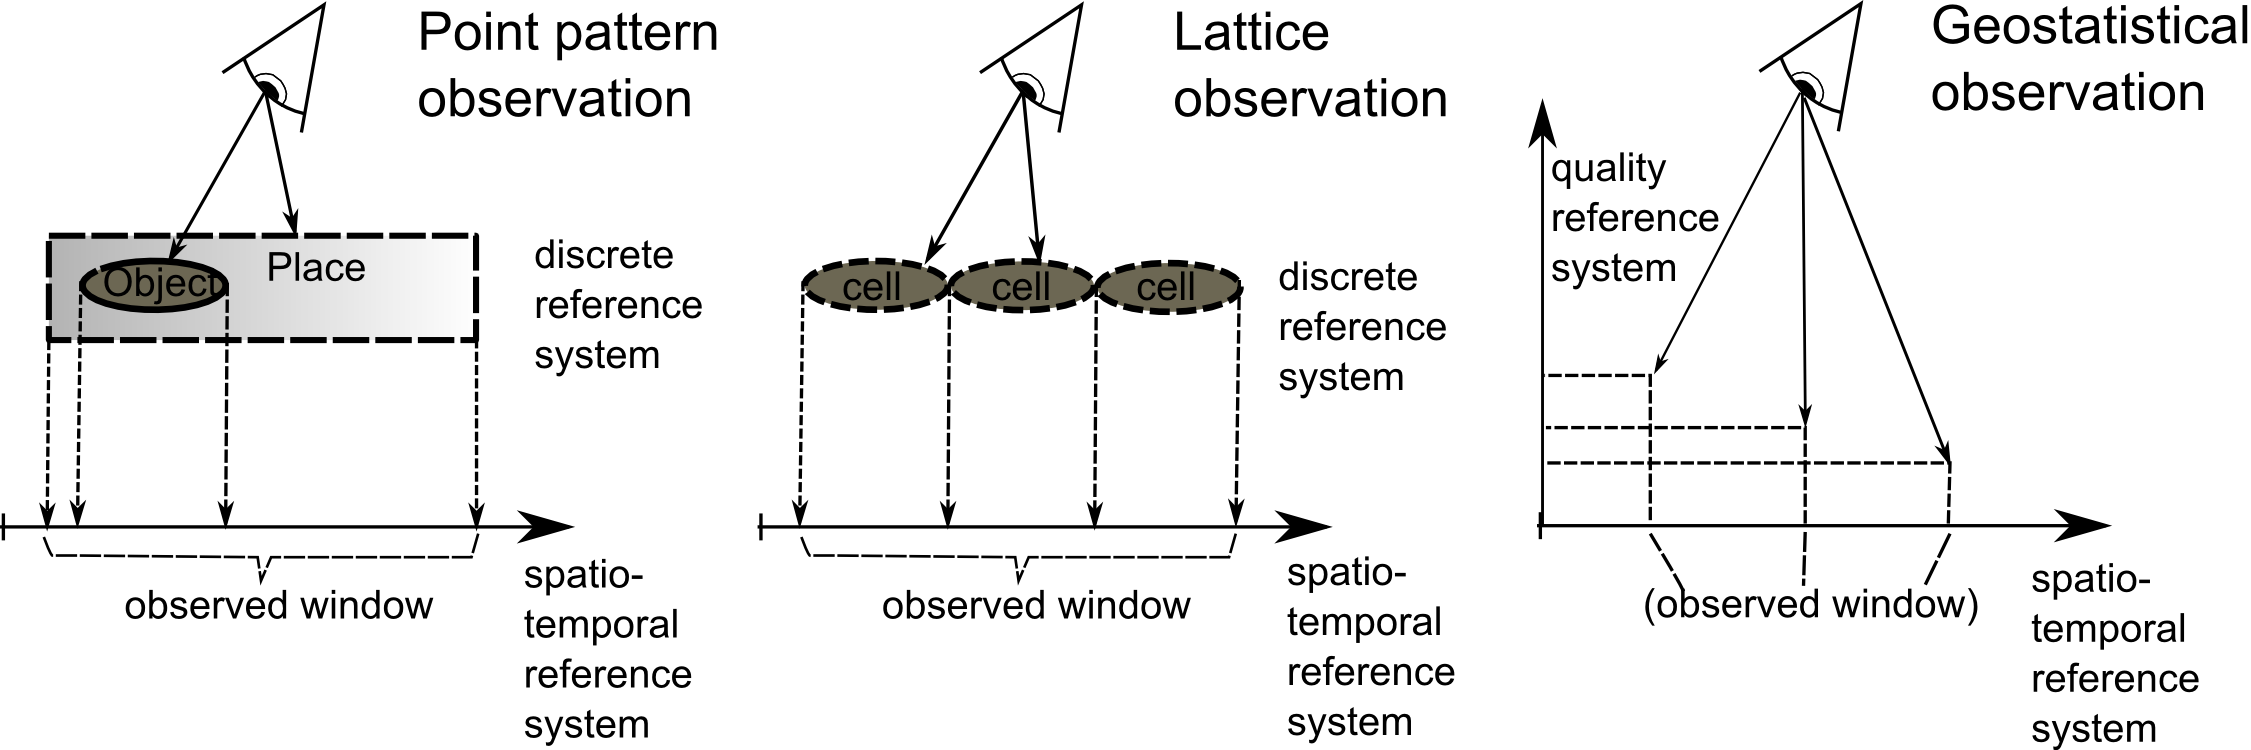
\includegraphics[width=1\textwidth]{observationwindow.png}
	\caption{Different Types of Observations and their Observed Window.}
	\label{fig:observationwindow}
\end{figure}

It is important to know that objects, such as animals, occured or did not occur within an area, or whether there are knowledge gaps. Observers know this because their window of attention can focus on whole places and they can detect all objects of a type in them (Figure \ref{fig:observationwindow}). In order to represent this knowledge in our formalism, the \textit{observed spatial window (${\it windowSpace}$)} is declared in Table \ref{tab:windows} as a mapping from a data set to a spatial region. For this region, the dataset encodes \textit{complete knowledge} about \textit{whether or not the underlying phenomenon occurred while he was observing}. That is, the observer knows that in the space inside this regions which is  not covered by data the phenomenon did not occcur. Analogously, the \textit{observed temporal window (${\it windowTime}$)} is defined as mapping from data to some temporal region, for which the data set encodes complete knowledge.

\begin{table}[htb]
\caption{Observed Spatial and Temporal Window}
\label{tab:windows}
\begin{tabular}[h]{|p{2.5cm}|c|p{5cm}|}
			\hline
			\textbf{Window Type} & \textbf{Observation Window Function} &  \textbf{Example} \\
			\hline
			\textit{Observed Spatial Window} & ${\it windowSpace :: "OBSD \Rightarrow \prescript{r}{}D_{s}"}$ &  Area of Germany where coal power plants have been observed. \\
			\hline			
\textit{Observed Temporal Window} & ${\it windowTime :: "OBSD \Rightarrow \prescript{r}{}D_{t}"}$ & Year 2008 for which the total ${\it CO_2}$ emissions of coal power plants have been measured. \\
			\hline
\end{tabular}
\end{table}

Observed windows can be continuous and, thus, infinite. For example, the window is continuous in case the observer has focused his attention on a continuous phenomenon, e.g., an extended place or an object as a \textit{ chunk of space}. This is the case for point patterns (see Figure \ref{fig:observationwindow}) and  formalized in Axiom \ref{ax:infiniteSPPW}. Similarly, remote sensors, e.g., satellite sensors, can cover a continuous space by a finite number of cells. This is a case for lattice observation (Figure \ref{fig:observationwindow}). 

\begin{Axiom}
Non-finiteness of an observed spatial window of spatial point pattern data:\\
 " ${\it\forall}$ (f::${\it SPPD}$) s'. windowSpace f  = s' ${\it \rightarrow \neg}$ finite s'"
\label{ax:infiniteSPPW}
\end{Axiom}

However, in case the observer or sensor focused attention on point-like locations in a spatial reference system, the observed window is discrete. This is the case for geostatistical observations (see Figure \ref{fig:observationwindow}) and is formalized in Axiom \ref{ax:finiteGEOSTW}. In this latter case, the observed window coincides with the spatio-temporal domain of the data function (and can thus be left away). Whereas in the former case, the observed window is an important kind of information about a data set.

\begin{Axiom}
Finiteness of an observed spatial window of geostatistical data:\\
 " ${\it\forall}$ (f::${\it GEOSTD}$) s'. windowSpace f  = s' ${\it \rightarrow}$ finite s' "
\label{ax:finiteGEOSTW}
\end{Axiom}

\subsection{Meaningful Prediction}
\label{prediction}

Prediction is the act of generating (estimating) values at locations/times at which values are unknown. We suggest that \textit{meaningful prediction} requires that predictions are \textit{interpretable in terms of underlying observation procedures}. Thus, meaningful prediction can be defined (Definition \ref{def:meaningfulPred}) as the application of a prediction procedure to data derived by an observation procedure, such that the corresponding observation function is defined for each predicted value. In other words, meaningfulness requires that there is a possible observation for each predicted value:

\begin{definition}[Meaningful Prediction]
\label{def:meaningfulPred}
 MeaningfulPred :: "$('a \Rightarrow 'b \Rightarrow 'c) \Rightarrow ('a \Rightarrow 'b \Rightarrow 'c) \Rightarrow bool$" where 
 "MeaningfulPred pred obs  $\equiv \forall$  x y z.(pred  x y  = z) $\rightarrow$ (obs x y $\neq$ error)"
\end{definition}

This definition needs to be overloaded for different types of observation functions with differing arities. Definition \ref{def:meaningfulPred} is defined for binary function types such as $\it{GEOST}$. 

To test meaningfulness of a prediction more generally, over a given set of data with their annotated observation functions, the computational challenge lies in first generating all possible observation functions (which may be logical compositions of primitive ones), and then searching for one corresponding pair of prediction and observation function that satisfies Definition \ref{def:meaningfulPred}. In searching, one can easily skip all pairs in which functions have a different type, as they cannot satisfy the necessary condition. Automatic proofs can thus be reduced efficiently to those cases when functional types coincide. Even checking function types without generating logical compositions is very useful, since it restricts the set of \textit{possibly meaningful} predictions, and thus helps the user choose an adequate prediction procedure. 

In our example scenarios of $CO_2$ emissions of coal power plants and ${\it PM_{10}}$ concentrations, Definition \ref{def:meaningfulPred} allows to automatically determine whether a spatial interpolation such as ordinary kriging is meaningful or not based on comparing observation and prediction functions. Ordinary kriging interpolation is specified as the function ${\it pred_{geost}}$ of type \textit{GEOST} (see Table \ref{tab:prediction}) and, hence, is defined for all locations in continuous space and time. 

\begin{table}[htb]
\caption{Function for an ordinary Kriging procedures}
\label{tab:prediction}
\begin{tabular}[h]{|p{3.5cm}|c|p{5cm}|}
			\hline
			\textbf{Prediction procedure} & \textbf{Prediction Function} &  \textbf{Example} \\
			\hline
			\textit{Ordinary kriging procedure} & ${\it pred_{geost}}$ :: $GEOST$ &  Spatial interpolation of ${\it PM_{10}}$ measurements using ordinary kriging. \\
			\hline
\end{tabular}
\end{table}

How can we prove meaningfulness in these cases? By Axiom \ref{ax:totality}, the function ${\it obs_{cphen}}$ is defined, i.e., has a non-error response, for every tuple in its domain. This domain coincides with the domain of ${\it pred_{geost}}$. Thus, it follows immediately that the interpolation of ${\it PM_{10}}$ concentration measurements using ordinary kriging is meaningful according to Definition \ref{def:meaningfulPred}: 
\begin{theorem}[Meaningful Prediction]
\label{the:Meaningful}
"MeaningfulPred ${\it pred_{geost}}$  ${\it obs_{cphen}}$"
\end{theorem}

While the ordinary kriging interpolation of ${\it PM_{10}}$ concentrations is meaningful, interpolating ${\it CO_2}$ emissions from coal power plants becomes meaningless. How can we disprove meaningfulness? First, the available observation functions ${\it obs_{loc}}$ and  ${\it obs_{prop}}$ obviously cannot be meaningfully interpolated according to Definition \ref{def:meaningfulPred}, since their functional domains do not correspond to ${\it pred_{geost}}$. Second, we need to exclude the possibility that there is a derived observation function which may be meaningfully interpolated. For this purpose, we need to generate observation functions with a corresponding functional type.
In fact, the phenomenon of ${\it CO_2}$ emissions from coal power plants may be represented by a derived function ${\it obs_{geost*}}$ of the required type. For illustration of this issue, an observation function ${\it obs_{invloc}}$ is given in Definition \ref{def:obsInvLoc} that is the inverse of the object localisation function ${\it obs_{loc}}$. The function ${\it obs_{invloc}}$ returns a discrete object for a spatial location, if the discrete object is observed at the spatial location, and an error otherwise.

\begin{definition}
\label{def:obsInvLoc}
 ${\it obs_{invloc}}$ :: "$D_s \Rightarrow D_t \Rightarrow D_d$" where \\
 "${\it obs_{invloc}}$ s t $\equiv$ (if ($\exists!$ d. ${\it obs_{loc}}$ d t = s) then ($\iota$ d. (${\it obs_{loc}}$ d t = s)) else (error::$D_d$))"
\end{definition}

The observation function ${\it obs_{geost*}}$ is defined (Definition \ref{def:pseudoGeost}) as a composition of the inverse localisation observation ${\it obs_{invloc}}$ and the object property observation ${\it obs_{prop}}$. It represents the \textit{spatio-temporal occurrence} of ${\it CO_2}$ emissions from power plants. Note that the type of this function is not distinguishable from a geostatistical variable, namely a set of tuples of space, time and measured value. And in fact, there are cases where the phenomenon actually needs to be represented in this way, e.g., in a geographic map of emission values. This illustrates the semantic challenge, because the function now resembles a geostatistical function, i.e., a function to predict ${\it CO_2}$ emission values for continuous spatial locations. 
\begin{definition}
\label{def:pseudoGeost}
${\it obs_{geost*}}$ :: GEOST where \\
"${\it obs_{geost*}}$ s t $\equiv$ if (${\it obs_{invloc}} \neq$ error) then ($\iota$ q. ${\it obs_{prop}}$(${\it obs_{invloc}}$ s t) t = q) else (error::$D_q$)"
\end{definition}

However, note that in our formalism, the functional specifications of $obs_{prop}$ and $obs_{invloc}$ allow to make the necessary distinction: we can infer that the function $obs_{geost*}$ is not defined over the whole spatial domain $D_s$. Hence, predicting values with $pred_{geost}$ for $obs_{geost*}$ is not meaningful, as there are predicted values for locations in space and time where the underlying observation function is not defined (Theorem \ref{the:notMeaningful}):
\begin{theorem}[Meaningless Prediction]
\label{the:notMeaningful}
"$\neg$ MeaningfulPred ${\it pred_{geost}}$  ${\it obs_{geost*}}$"
\end{theorem}

The proof of Theorem \ref{the:notMeaningful} requires the whole formal mechanism introduced so far and is provided in \ref{appendix:theorem3proof}.

\subsection{Meaningful Aggregation}
\label{aggregation}

Spatio-temporal aggregation procedures describe how to generate lattice data from point pattern or geostatistical data. They consist of two steps: First, groups are composed according to spatio-temporal predicates, usually referred to as \textit{group composition}. Then, an aggregate value is computed for each group of objects. For example, the spatial grouping predicates for ${\it PM_{10}}$ observations might be containment in the federal states of Germany. Applying these grouping predicates to observation data sets results in groups of observations per each federal state. As we focus on the generation of lattice data from point data, the grouping predicates in our case correspond to spatial and/or temporal lattices. 

Summing a quality that is distributed in space requires that the quality has been observed completely over the extent over which it should be aggregated. This is the case for a marked point pattern aggregated on a lattice that is covered by its observed window. However, it is not the case for geostatistical data, as it is not possible to gather observations at continuous locations. Hence, we do not know about unobserved places in the lattice, and thus are not able to compute a meaningful sum. 

We can formalize meaningful summation in Definition \ref{def:meaningfulSum} by utilizing our definition of the observed window (Table \ref{tab:windows}). Applying the sum to compute aggregates from data is meaningful, if all locations in the lattice are also part of the observed window. This condition ensures that the lattice regions have been observed completely.

\begin{definition}[Meaningful Summation:]  
	MeaningfulSum :: "DATA $\Rightarrow$ SR $\Rightarrow$ bool" where\\
"MeaningfulSum (data:: DATA) (lat::SR) $\equiv$ (Lattice lat)  $\wedge$ \\
($\forall$ (x::$D_s$) x'. (lat x' $\wedge$ x $\in$ x'   $\rightarrow$ (x $\in$ windowSpace(data))))"
\label{def:meaningfulSum}
\end{definition}

With Definition \ref{def:meaningfulSum} and the axioms and definitions introduced so far, it can be proved that summation of ${\it data_{geost}}$ to regions in ${\it slattice}$ is not meaningful. The proof of Theorem \ref{the:notMeaningfulSum} is explained in Annex \ref{appendix:notMeaningfulSum}.
\begin{theorem}[Meaningless Summation]
\label{the:notMeaningfulSum}
"$\neg$ MeaningfulSum ${\it data_{geost}}$ slattice"
\end{theorem}
 
For meaningfulness of other aggregation functions than the sum, one can utilize measurement scales. As an example, we are using the classification of Stevens \citep{Stevens1946} in nominal, ordinal, interval and ratio scale in order to find permissable descriptive statistics as shown in table \ref{measScalesTable}. Point pattern processes can be considered as nominal values, as they are pointing to locations for a certain type of objects or events, for example positions of Pine trees or of earthquakes. Thus, the only applicable aggregation function is count. In case of marked point patterns with nominal marks, an applicable statistic is mode, e.g. in case of different tree species the dominant species in a certain area. Marks of point patterns, and observed values of geostatistical or lattice variables can be of any scale type, and hence aggregation functions can be applied as shown in table \ref{measScalesTable}. This allows, for example, to compute the mean for geostatistical variables. However, the aggregates are only relevant in the context of the observed window.

\begin{table}
\caption{Types of Measurement Scales and Permissible statistics (after \citep{Stevens1946});
statistics permissible for lower scales are also permissible for higher scale variables, but not vice-versa.}
\label{measScalesTable}
\begin{tabular}[h]{|p{3cm}|p{9cm}|}
			\hline
			\textbf{Scale Type} & \textbf{Permissible Statistics} \\
			\hline
			\textit{Nominal} & Count (number of cases), Mode, Contingency \\
			  \hline
			  \textit{Ordinal} & Median, Percentiles \\
			  \hline
			  \textit{Interval} & Mean, Standard Deviation, rank-order correlation, product-moment correlation \\
			  \hline
			  \textit{Ratio} & Coefficient of variation \\
			  \hline
\end{tabular}
\end{table}

\section{Implementation} \label{implementation}

A prototypical implementation of our approach is provided for the R software that is a widely used statistical software environment \citep{R}. R also allows for spatial statistical analysis through several R packages that extend the R's core functionality \citep{Bivand2008}. However, at the moment, the different spatial packages do not restrict models to particular variable types. It is, for example, possible to apply an inverse distance interpolation to marked point patterns in the spatstat R package. The result of such an interpolation is shown in Figure \ref{fig:llpinesIdw}. 

\begin{figure}[ht]
	\centering
		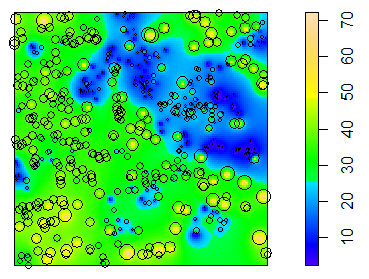
\includegraphics[scale=0.7]{llpines_idw.png}
	\caption{Interpolated marked point pattern (diameters of longleaf pines) with R package spatstat.}
	\label{fig:llpinesIdw}
\end{figure}

In order to disallow or allow particular interpolation and aggregation methods, we extend the sp package of R \citep{Pebesma2005} as shown in Figure \ref{fig:subclassesR}\footnote{The R script is available online at \url{https://svn.52north.org/svn/geostatistics/main/meaningful/tools/R/implementation.R}.}. The classes PointPatternDataFrame and GeostatisticalDataFrame extend the SpatialPointsDataFrame and the class LatticeDataFrame extends the SpatialPolygonsDataFrame. The subclass PointPatternDataFrame has an additional property observedWindow that represents the observed window as defined in our formalism (Section \ref{data}) and is of type SpatialPolygons. 

\begin{figure}[ht]
	\centering
		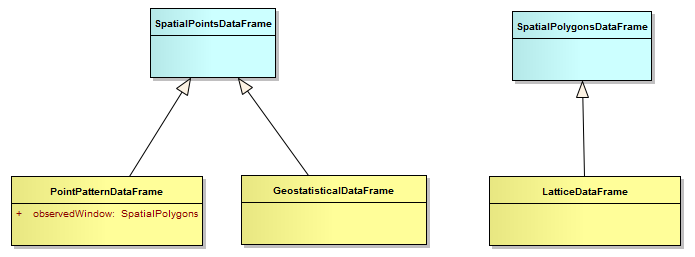
\includegraphics[scale=0.7]{imp_subclasses.png}
	\caption{Subclasses of the sp package classes used for meaningful interpolation and aggregation. The PointPatternDataFrame and GeostatisticalDataFrame classes are subclasses of the SpatialPointsDataFrame, the LatticeDataFrame class is subclass of the SpatialPolygonsDataFrame. Classes of package sp are shown as blue boxes, classes added in the prototypical implementation are shown as yellow boxes. Regular lattices such as remote sensing imagery is formally a subclass of LatticeDataFrame, but will in practice be implemented as a subclass of SpatialGridDataFrame or RasterStack.}
	\label{fig:subclassesR}
\end{figure}

Encouraging or discouraging aggregations and predictions is now implemented as a simple type-checking according to our formalism. The generic \lstinline|aggregation| function is augmented for the \lstinline|PointPatternDataFrame| and \lstinline|GeostatisticalDataFrame| classes. In case a non-meaningful interpolation is applied, i.e., spatial interpolation is applied to data of a \lstinline|PointatternDataFrame|, a warning message is printed in the console as shown in Figure \ref{fig:aggWarning}. 

\begin{figure}[ht]
	\centering
		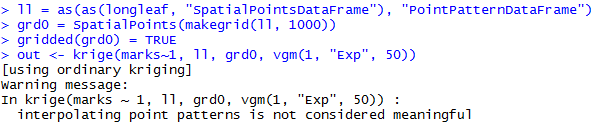
\includegraphics[scale=0.6]{warningMessage.png}
	\caption{Warning message in R console in case of a non-meaningful interpolation function.}
	\label{fig:aggWarning}
\end{figure}

In addition to the R implementation, a preliminary version of the theory's types as an ontology pattern in OWL is published on the Web\footnote{The pattern is available online at \url{http://www.meaningfulspatialstatistics.org/theories/MeaningfulSpatialStatistics.owl}. A diagram of the pattern is available online at \url{http://www.meaningfulspatialstatistics.org/theories/MeaningfulSpatialStatistics}.}. It can be utilized to implement our approach not just for the R software, but also for other tools such as ArcGIS or Web services defined by the Open Geospatial Consortium as illustrated in Figure \ref{fig:owlPattern}. Semantic anntotations referencing the concepts in the OWL pattern can be added to datasets as described by \cite{Janowicz2010}. OWL reasoners can be used to automatically determine which type of function has generated the data and which predictions or aggregations are applicable, based on type checks with subsumption reasoning. This replaces the issue of a manual declaration (see Figure \ref{fig:aggWarning}, first line in code) and of implementing type-based meaningfulness checks within each particular tool, enabling the creation of smarter data instead of smarter applications.

\begin{figure}[ht]
	\centering
		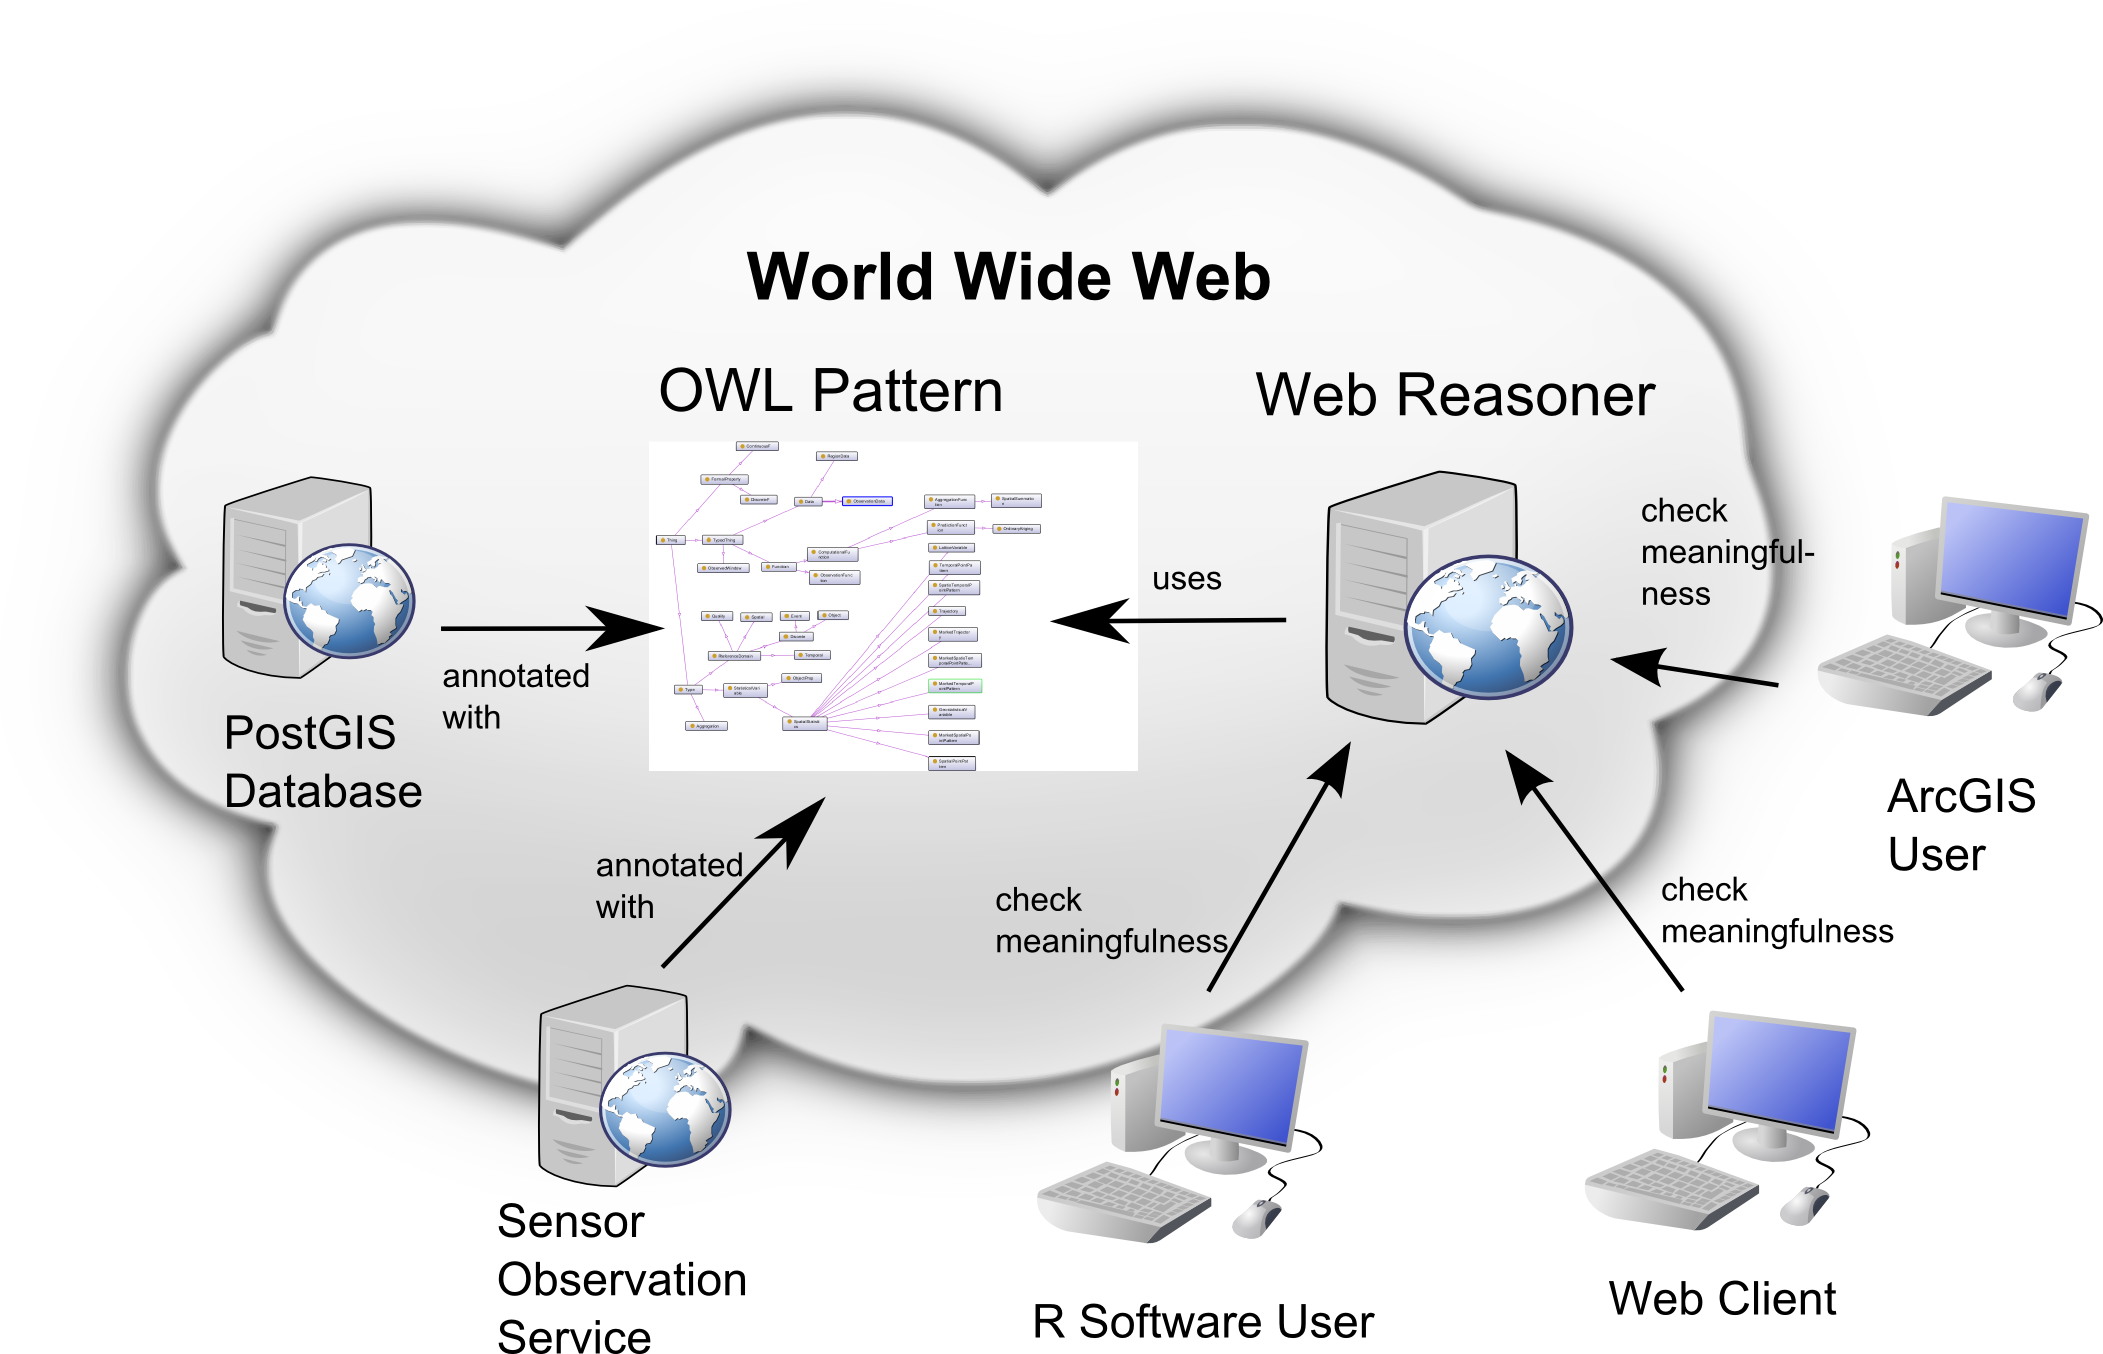
\includegraphics[scale=0.7]{owlPatternApp.png}
	\caption{Illustration of the use of the OWL pattern. Data available in the Web through, for example, Sensor Observation Services or database servers may be annotated with the types defined in our formalism. Different tools such as R, ArcGIS or general Web clients may use these annotations and a Web reasoner to automatically determine meaningful aggregation or prediction procedures.}
	\label{fig:owlPattern}
\end{figure}

\section{Discussion}\label{discussion}

Due to the increasing variety and volume of data sources which have to be dealt with in automatic systems that support prediction and analysis, it becomes necessary to take the semantics of models and data explicitly into account in order to support data-model interoperability \citep{Bell2009,Parsons2011}. In this paper, we present a formal theory for meaningfulness of spatial prediction and aggregation that addresses this interoperability problem. We consider it as a first step towards recommender tools for spatio-temporal modeling. 

In order to be used as a recommender service, the formal check of meaningfulness, which was performed in this paper in a semi-automated fashion, needs to be performed by \textit{tractable} automated reasoning tools that allow to be used on the Web or in statistical software, since higher-order logic (HOL) reasoning is not decidable. The challenge therefore consists in constraining the reasoning problem, the  matching of functions and data sets, sufficiently as to be fully automated. In this paper, we have made some suggestions and started with a preliminary recommender system based only on type-checks for spatial data in R \citep{Pebesma2005}. It guides the users of spatial data in the application of appropriate aggregation and interpolation methods. While a first version of an OWL pattern representing the types defined in our formalism is available in the Web, further work needs to be done to implement the pattern in the Web as shown in Figure \ref{fig:owlPattern}.

In our approach, data needs to be classified as representing either (marked) point patterns, geostatistical, or lattice variables. We are aware that this is not a deterministic decision and there is a large \textit{degree of freedom} in semantic conceptualization (compare the discussion in \cite{Scheider.2011c}, Chapter 4). This is also related to the well-known distinction between object-based and field-based approaches in GIS, which is a matter of information purpose and design \citep{Couclelis.92} as well as observation \citep{Frank2009}. Our formal framework serves to make this decision explicit and transparent.

Since our approach explicitly takes into account data abstraction procedures, data at point support in a spatial reference system with a certain granularity might also be represented by spatial and/or temporal regions in another reference system with finer granularity. We have proposed to include the observed window in the observation procedure description, and shown how aggregation can be used to convert from one granularity to another.

Information about the sampling procedure might be of importance for statistical modeling, e.g., whether design-based methods can be applied \citep{Gruijter2006}. This kind of information was not included in this paper, but may be incorporated in the observation procedure description and then used as additional information for reasoning about the meaningfulness of a particular prediction or aggregation.

Our notion of meaningfulness in aggregation requires that the regions over which data should be summed needs to be observed completely. In the OLAP and Statistical database community, several authors try to address the issue of summarizability as well \citep{Lenz1997,Mazon2009,Niemi2010} and also define a completeness condition. However, their definition of completeness states that each non-aggregated observation needs to be covered by at least one region. Instead, we require that knowledge is needed for the whole region over which data should be summed, which is the case for point pattern variables, but not for geostatistical variables. Our approach for spatio-temporal aggregation can be seen as a complementary contribution to this issue, as the work on the summarizability so far does not explicitly consider different types of spatial variables. 

In our approach, we focus on the aggregation of point data (either point patterns or geostatistical variables) to areal data. However, the resulting areal data might be, in turn, aggregated to larger areas and so forth. It appears that the distinction between point patterns (i.e. discrete entities that are represented by some space-time geometry) and geostatistical variables (continuous phenomena in space/time) is still valid also for areal data. As an example, the sum of discrete entities still makes sense for areal data, e.g. summing the total CO2 emissions of power plants per each European country to the sum of Europe, while summing the temperature appears still not appropriate for polygonal data.

An example of an aggregation of the air quality variable PM$_{10}$ is shown in Figure \ref{eea}, which was published by the \cite{eea}. In this report, a section on {\em Europe-wide survey of PM} shows time trends in PM$_{10}$ concentrations averaged over monitoring network stations with complete measurement records. Below the figure it notes that {\em ``in the diagrams a geographical bias exists towards central Europe where there is a higher density of stations''}, but it is not made clear whether this bias refers to selection, to estimation, or both. We argue that these trends relate to the stations selected, rather than an area (Europe). Areal mean values can be predicted, e.g.~by block kriging \citep{Journel1978}. 

\begin{figure}
\begin{center}
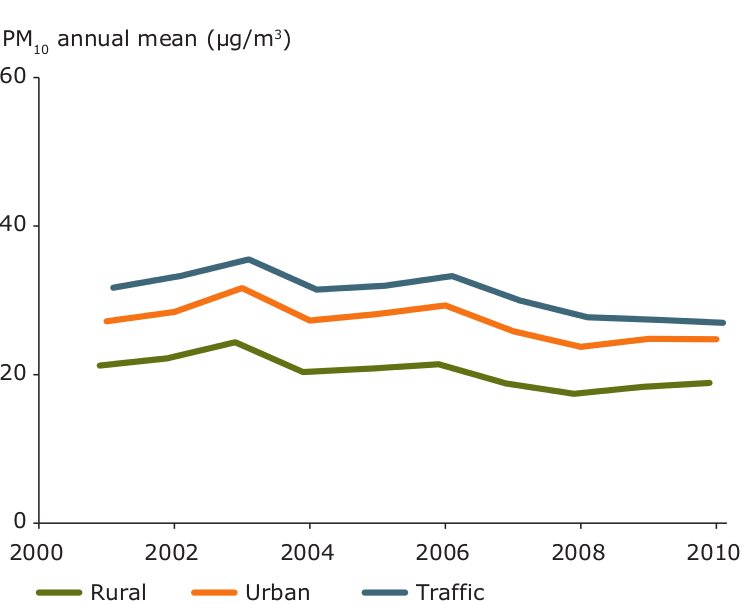
\includegraphics[width=0.6\columnwidth]{pm10.png}
\end{center}
\caption{ Trends in PM$_{10}$ ($\mu g / m^3$), 2001-2010, per station type.
Source: \cite{eea}}
\label{eea}
\end{figure}

While we have proposed meaningfulness of predictions based on reference systems, we have not yet considered meaningfulness of statistical models.  An example is the decision for which area we may assume second order stationarity of a phenomenon. Interpolating PM$_{10}$ values measured at traffic stations (figure \ref{eea}) to areas with rural, traffic-free conditions (and vice versa) may not be meaningful. Towards such meaningful models, further work is needed to determine and formalize the additional required information. Our approach can be a starting point towards choosing such meaningful models. In the context of evaluating model performance \citep{Bennett2013}, our theory covers meaningfulness of spatial prediction and aggregation of model residuals. Furthermore, we do not include semantic descriptions of concrete application problems. An example of this would be predicting air quality over Beijing. The formalization of this application problem would allow matching appropriate data and prediction procedures with the application goal.

For meaningfulness of other aggregation functions than the sum, we are using Stevens' classification scheme \citep{Stevens1946} and emphasize that point patterns might be considered as nominal data, whereas the application of statistical measures to marked point patterns, geostatistical and lattice data depends on the measurement scale of the quality values that are observed. As pointed out by several authors \citep{Suppes1967,Hand1996,Chrisman1995}, Stevens' classification of four measurement scale types is quite limited and there are several other types of measurement scales. For example, \cite{Chrisman1995} proposes an extended framework for geographical measurement, which introduces additional measurement scale types (e.g. cyclic scale or absolute scale for probabilities) and which incorporates information whether space, time, or attributes have been fixed during the measurements. His work is based on earlier work of Sinton who distinguishes different variables related to its representation in thematic maps \citep{Sinton1978}. Similarly, we distinguish the different variable types in Spatial Statistics based upon fixed domains and those being considered as the result of a random process and show how these affect the meaningfulness of aggregation in case of using the sum as aggregation function. While we believe, that, in general, the other permissable statistics in Stevens' classification are meaningful for quality domains of marked point patterns and geostatistical data, more work needs to be done to examine other common aggregation functions and their meaningfulness regarding specific variable types and reference domains. Furthermore, different measurement scale types allow for different representations of the same process: The occurence of longleaf pines can be represented as a point pattern (nominal scale) or as a Geostatistical variable with binary scale (false, if there are no pines, true otherwise) or as an absolute scale [0,1] showing the probability of longleaf pines presence as a derived measurement.

Finally, one might have concerns and argue that data exploration is always dealing with finding the unexpected and that the application of particular prediction or aggregation methods should not be restricted at all. While we, in general, agree that methods should not be disallowed, we believe that support on finding appropriate methods, and warnings in case inappropriate methods are applied, is useful as it increases awareness on the risk of drawing false conclusions due to inappropriate use of predictions or aggregations.


\section{Conclusion}\label{conclusions}

We introduced a new notion of meaningfulness of prediction and aggregation and formally specified it in a semantic theory in higher order logic (HOL). The theory consists of functional specifications of observation procedures, prediction procedures, aggregation procedures, as well as datasets based on semantic reference systems as types. Our notion of meaningfulness is based on the formal distinction between observation, prediction, and aggregation \textit{procedures} on the one hand, which describe potential data, and \textit{data} on the other hand, which is generated by executing these procedures. The different procedures are represented as functions of different types, which correspond to known variable types in Spatial Statistics. Data are represented by predicates on the domain and range of these functions, i.e., they are a finite subset of the tuples defined by a function. Meaningfulness checks are implemented in our formalism as \textit{correspondence checks}: \textit{Meaningful prediction} is introduced based on a correspondence check between observation functions and prediction functions that ensures that there is a possible observation for each prediction. \textit{Meaningful aggregation} is based on checking whether an observed window corresponds to the target regions of an aggregation, hence testing the condition, that the target region needs to be observed completely in case of using the sum as an aggregation function. The theory, including definitions, axioms, and theorems, was implemented and tested with Isabelle/HOL, a semi-automated theory prover.

One challenge for future work consists in tractable implementations of meaningfulness checks in open Semantic Web environments as well as in statistical software. As environmental models always deal with uncertain data \citep{Bastin2013}, and since uncertainty can be seen as a consequence of observation \citep{Frank2009}, its inclusion in our formalism would be natural. Future work may also address the extension of our theory to cover other related notions of meaningfulness, the incorporation of sampling procedures, other types of aggregation and prediction, as well as further measurement scales.

\section*{Acknowledgments}
The presented work was developed within the 52$^\circ$ North geostatistics community, and partly funded by the European project UncertWeb (FP7-248488, see http://www.uncertweb.org/) and the International Research Training Group on Semantic Integration of Geospatial Information funded by the DFG (German Research Foundation), GRK 1498.
Simon Scheider's contribution was partly funded by a research fellowship grant (DFG SCHE 1796/1-1) and the ICT-FP7-249120 ENVISION project.

\bibliographystyle{model2-names}
\bibliography{mip}

\appendix

\section{Cardinality Order on Types}
\label{appendix:sortCardinality}

\textit{Partial cardinality orders} among domains can be formalized based on the existence of \textit{embeddings}, i.e., injective total functions $f:X\Rightarrow Y$ from type $X$ into the one with higher cardinality $Y$. Partial cardinality order on types,  ${\it X \subseteq_{c} Y}$, thus, can be expressed in Isabelle as follows:
 $$
{\it \exists (f:: X \Rightarrow Y). inj\; f}
$$
\label{subseteqc1}
A \textit{strict} cardinality order $X \subset_{c} Y$ can be formalized accordingly by requiring that \textit{all mappings} ${\it f::X\Rightarrow Y}$ are \textit{non-surjective}, i.e., they do not fully cover $Y$. We formally capture this by an axiom that denies surjectivity:
  \begin{Axiom}
Strict cardinality order on reference domains:\\
 ${\it 
 \neg (\exists (f::D_d \Rightarrow D_s). surj\; f)}$\\
 ${\it \neg (\exists (f::D_d \Rightarrow D_t). surj\; f) }$
\label{subseteqc}
\end{Axiom}
Which is how we translate the cardinality differences ${\it D_d \subset_{c} D_s \wedge D_d \subset_{c} D_t}$ into Isabelle.

\section{Proof of Theorem \ref{the:notMeaningful}}
\label{appendix:theorem3proof}

In order to prove that the prediction of ${\it CO_2}$ emissions of coal power plants, represented by ${\it obs_{geost*}}$, with an Ordinary Kriging interpolation procedure, represented by ${\it pred_{geost}}$, is not meaningful (Theorem \ref{the:notMeaningful}), it needs to be shown that Definition \ref{def:meaningfulPred} is not satisfied by the functions ${\it obs_{geost*}}$ and ${\it pred_{geost}}$, i.e., that there are spatial and temporal locations at which the predicition function provides a quality value, but where the corresponding observation function returns an error. The following is a description of substeps of the automated proof which is available online\footnote{\url{http://www.meaningfulspatialstatistics.org/theories/Miptheory.thy}.}.

\begin{proof}
First, using Axiom \ref{subseteqc} and the definition of surjectivity, it can be proved that all functions of type $D_d \Rightarrow D_s$ (mappings from discrete entities into space) miss some entity in their range as specified in Theorem \ref{the:nonSurjectivity}. 
\begin{theorem}
\label{the:nonSurjectivity}
Non-surjectivity of object-space mappings:  "$\forall$ (f:: $D_d \Rightarrow D_s$).($\exists$ (s::$D_s$).$ \neg $( $ \exists $ (d::$D_d$). s = f d))"
\end{theorem}

Using only Theorem \ref{the:nonSurjectivity}, it can be directly proved that the object localisation function ${\it obs_{loc}}$ misses entities in its range at all times (Theorem \ref{the:nsObsLoc}):
\begin{theorem}
\label{the:nsObsLoc}
Non-surjectivity of ${\it obs_{loc}}$: " $\forall$ t.($\exists$ s.$\neg$($\exists$ d. s = ${\it obs_{loc}}$ d t))"
\end{theorem}

Hence, using Definition \ref{def:obsInvLoc} and Theorem \ref{the:nsObsLoc}, it can be proved that the inverse function ${\it obs_{invloc}}$ generates errors for some spatial locations at all times:
\begin{theorem}
\label{the:nsInvObsLoc}
Errors in ${\it obs_{invloc}}$: "$\forall$ t. ($\exists$ s. ${\it obs_{invloc}}$ s t = error)"
\end{theorem}

Thus, the pseudo-geostatistical observation function ${\it obs_{geost*}}$ produces errors, too, as it is constructed with ${\it obs_{invloc}}$. This can be proved by Theorem \ref{the:nsInvObsLoc} and Definition \ref{def:pseudoGeost}:
\begin{theorem}
\label{the:errorsPseudoGeost}
Errors in ${\it obs_{geost*}}$:  "($\exists$ y x. ${\it obs_{geost*}}$ x y = error)
\end{theorem}

Hence, the domain of ${\it obs_{geost*}}$ is of lower cardinality, i.e., defined only for a true discrete subset of $D_s$, reflecting the fact that ${\it CO_2}$ emissions (in contrast to concentration) need emitters that are discrete objects (coal power plants). Thus, there are predictions that are not paralleled by any observation. Our goal was to show that predicting ${\it obs_{geost*}}$ with ${\it pred_{geost}}$ is not meaningful (Theorem \ref{the:notMeaningful}). This follows immedately from Theorem \ref{the:errorsPseudoGeost} and Definition \ref{def:meaningfulPred}.
\end{proof}

\section{Proof of Theorem \ref{the:notMeaningfulSum}}
\label{appendix:notMeaningfulSum}

In order to show that the computation of a sum of geostatistical values, such as ${\it data_{geost}}$, over spatial lattices, such as ${\it slattice}$, is not meaningful (Theorem \ref{the:notMeaningfulSum}), we need to show that there exist locations in the spatial lattice that are not contained in the observed window of the observation data, corresponding to Definition \ref{def:meaningfulSum}. The following is a description of substeps of the automated proof which is available online\footnote{\url{http://www.meaningfulspatialstatistics.org/theories/Miptheory.thy}}.

\begin{proof}
First, based on Axiom \ref{ax:finiteGEOSTW}, we infer that the observed spatial window of ${\it data_{geost}}$ needs to be finite:
\begin{theorem}
\label{the:finitSwGeost}
Finiteness of observed spatial window of ${\it data_{geost}}$: \\"finite (windowSpace ${\it data_{geost}}$ )"
\end{theorem}

In addition, based on Axioms \ref{ax:latticeProps} and \ref{ax:dataGeost}, we can prove that regions in the spatial lattice ${\it slattice}$ are not finite (actually, they are continuous sets of points):  
\begin{theorem}
\label{the:infinitLatReg}
Non-finiteness of lattice regions: \\"$\forall$ x. slattice x $\rightarrow$ $\neg$ finite x"
\end{theorem}

Using the very same axioms together with Definition \ref{def:dataFiniteness} for data properties, it can also be shown that there is at least one region in \textit{slattice}.
\begin{theorem}
\label{the:exLatReg}
Existence of region in slattice: \\"$\exists$ x. slattice x"
\end{theorem}

From Theorems \ref{the:finitSwGeost}, \ref{the:infinitLatReg}, and Axiom \ref{ax:finitenessundinfinity}, it follows that there is a spatial location in a region of the spatial lattice that is not part of the observed spatial window of ${\it data_{geost}}$ : 
\begin{theorem}
\label{the:cardinality}
Cardinality of observed window and regions: "$\forall$ x. slattice x  $\rightarrow$($\exists$ z. (z $\in$ x) \& $\neg$(z: windowSpace ${\it data_{geost}}$ ))"
\end{theorem}

Hence, the observed spatial window of ${\it data_{geost}}$ is of lower cardinality than the regions in \textit{slattice}. Theorems \ref{the:cardinality} and \ref{the:exLatReg} together with Definition \ref{def:meaningfulSum} for meaningful sum allow to derive Theorem \ref{the:notMeaningfulSum} immediately.
\end{proof}

\end{document}

